\section{Progettazione e codifica}

A partire dalle specifiche fornite dal committente, è stata svolta una accurata analisi per scomporre il questionario di oltre mille domande in questionari di dimensione minore e direttamente correlati alla risorsa di pertinenza.\\
In particolare sono state oggetto di analisi le seguenti componenti:
\begin{itemize}
	\item \textit{Figure di sistema;}
	\item \textit{Dispositivi di protezione individuale;}
	\item \textit{Mansioni;}
	\item \textit{Formazioni;}
	\item \textit{Questionari;}
	\item \textit{Segnalazioni;}
	\item \textit{Procedure;}
	\item \textit{Dispositivi di protezione collettivi.}
\end{itemize}
Per ogni componente, è stato realizzato o restaurato il modello corrispondente, aggiornate le viste che ne facevano uso. Sono state implementate inoltre le regole Drools per verificare la conformità delle informazioni inserite alle norme vigenti in ambito di sicurezza.
\subsection{Riprogettazione delle componenti esistenti}
	
	
\subsubsection{Riprogettazione della componente: \textit{Figure di sistema}}

	Con \textit{figure di sistema} si intendono tutte le cariche che hanno la responsabilità di garantire la sicurezza in azienda. \\
	Come specificato dal testo unico della salute e sicurezza sul lavoro (D.lgs. 81/2008), esse sono: 
	\begin{itemize}
		\item Datore di lavoro;
		\item Dirigente;
		\item Preposto;
		\item Medico Competente;
		\item Responsabile del servizio di prevenzione e Protezione (RSPP);
		\item Addetto al servizio di prevenzione e Protezione (ASPP);
		\item Responsabile dei Lavoratori per la Sicurezza (RLS).
	\end{itemize}
	L'operato delle figure sopra elencate deve essere supervisionato da un \textit{Organo di vigilanza}.

	\paragraph*{Situazione precedente alla riprogettazione} \mbox{} \\
	
	La situazione iniziale prevedeva che la classe \textit{Individual} avesse  un attributo booleano per ogni tipologia di figura di sistema. \\
	Si è resa necessaria una riprogettazione dal momento che alcune figure dovevano ricoprire lo stesso ruolo contemporaneamente in più contesti e questa situazione non poteva essere gestita con l'architettura esistente. \\
	Un esempio di tale problema è rappresentato da un ASPP assegnato a due cantieri contemporaneamente. Tale situazione si può verificare se i due cantieri sono allocati nello stesso periodo e nel primo si lavora il mattino, mentre nel secondo di pomeriggio oppure a giorni alterni.\\
	I questionari relativi a a tutte le figure di sistema erano presentati in una pagina contenente tutte le domande. I problemi che tale soluzione procurava erano sostanzialmente due: era possibile gestire al più un individuo per ogni ruolo e le domande a cui rispondere in una sola sezione erano più di centocinquanta.

	\paragraph*{Modifiche apportate}\mbox{} \\
	L'architettura è stata riprogettata centralizzando tutti i ruoli in una apposita classe \texttt{Role} e Mantenendo la relazione molti a molti mediante una tabella intermedia \texttt{IndividualRoles}. \\
	Questo approccio si è rivelato molto vantaggioso perché ha permesso di associare ogni classe rappresentante un ruolo, alle formazioni minime che un individuo deve possedere per poter ricoprire quella carica. \\
	Questa soluzione (\autoref{fig:DiagrammaDelleClassiIndividualRoles}) soddisfa appieno tutti ri requisiti.\\
		\begin{figure}[H]
			\begin{center}
				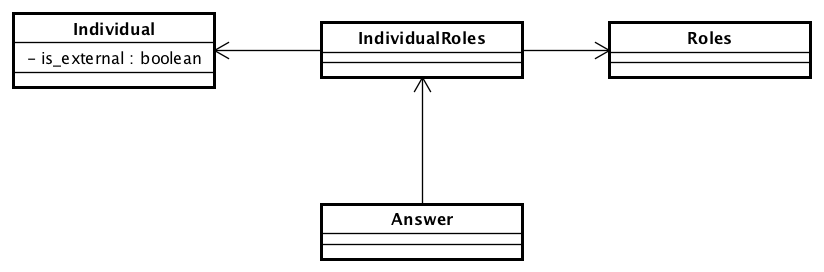
\includegraphics[width=12cm]{Pics/UMLClassiFigureDiSistema.png}
				\caption{
					Diagramma delle classi per la gestione delle figure di sistema ed i relativi questionari.}
				\label{fig:DiagrammaDelleClassiIndividualRoles}
			\end{center}
		\end{figure}
	Obiettivo primario della riprogettazione è stato centralizzare tutte le informazioni relative alle figure di sistema ed i loro questionari in un unica sezione. 
	La schermata presente nella  \autoref{fig:ScreenPrincipaleFigureDiSistema} vuole rappresentare il risultato del lavoro svolto per le figure riguardanti l'azienda. \\
		\begin{figure}[H]
			\begin{center}
				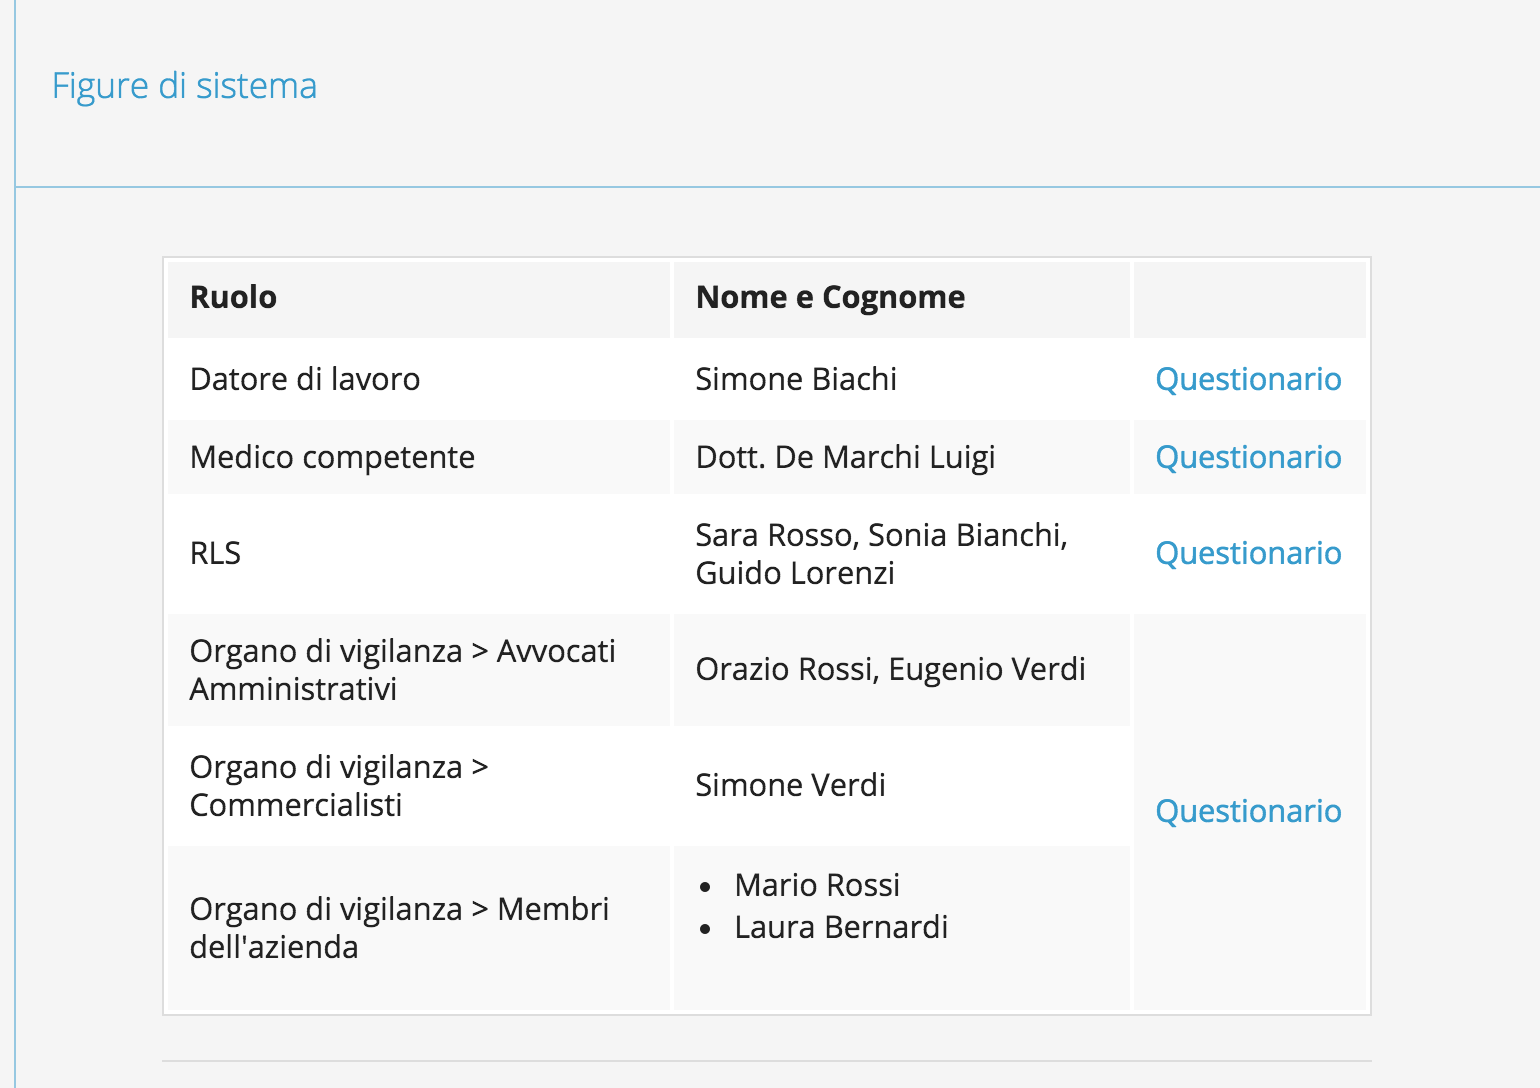
\includegraphics[width=12cm]{Pics/ScreenFigureDiSistemaProspetto.png}
				\caption{
					Schermata iniziale della sezione \textit{Figure di sistema}.}
				\label{fig:ScreenPrincipaleFigureDiSistema}
			\end{center}
		\end{figure}
	È stato implementato inoltre un pannello dedicato alla gestione delle figure impiegate in specifiche sedi o cantieri. In questo modo è sempre possibile allocare gli individui nei luoghi d'interesse senza vincoli di molteplicità.\\
	\begin{figure}[H]
		\begin{center}
			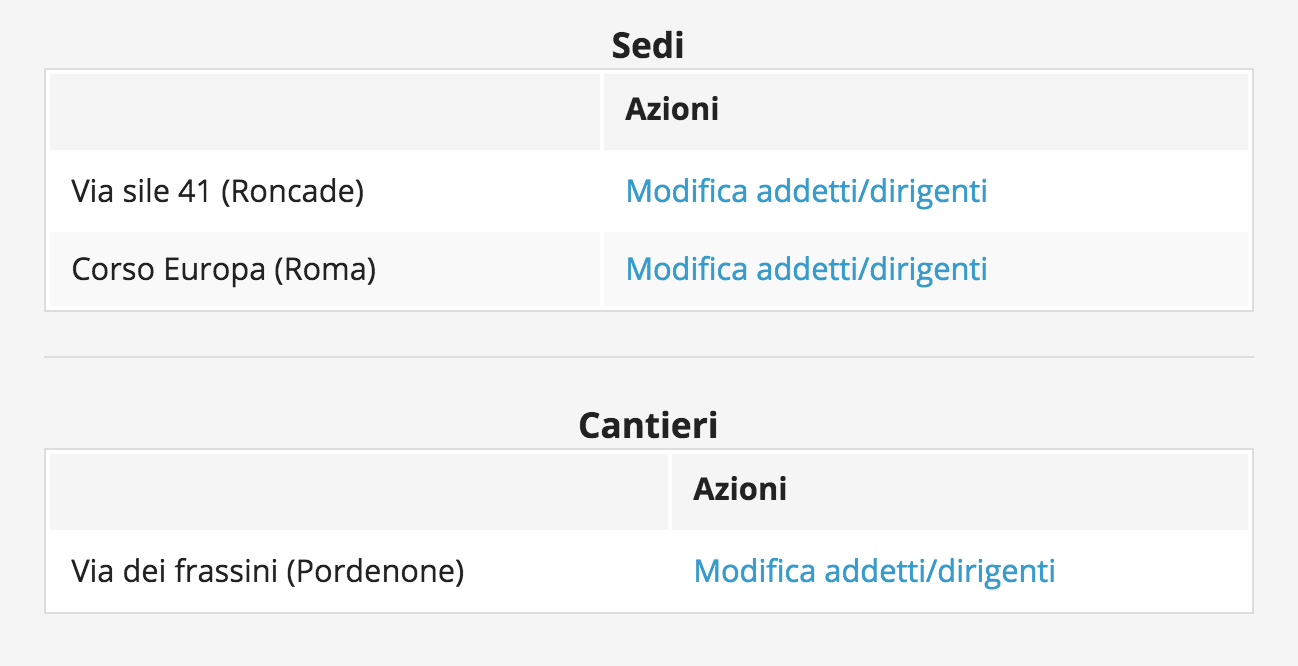
\includegraphics[width=12cm]{Pics/ScreenfigureDiCantiere.png}
			\caption{
				Schermata iniziale della sezione \textit{Pannnello di gestione delle figure impegnate in sedi e cantieri.}.}
			\label{fig:ScreenPrincipaleFigureSediCantieri}
		\end{center}
	\end{figure}

	Per facilitare l'inserimento delle informazioni relative alla selezione dei dipendenti, è stata utilizzata la libreria \textit{Selectize.js} per rendere i form più gradevoli dal punto di vista grafico e per permettere l'autocompletamento (vedi \autoref{fig:ScreenOrganodiVigilanza} ). \\ 
	Una criticità si è presentata nell'inserimento dinamico delle figure che possono essere presenti con molteplicità maggiore di uno. In particolare gli RSPP e gli ASPP presentano l'ulteriore complicazione rappresentata dal fatto che possono essere sia membri interni all'azienda, sia esterni. \\
	In entrambi i casi, la situazione è stata gestita mediante chiamate \gls{Ajax}, evitando quindi di dover ricaricare la pagina ad ogni inserimento e generando un record della classe \textit{Individual}  identificato da un particolare flag (\texttt{is\_external}) nel caso si tratti di una figura esterna all'azienda.\\
	
	\begin{figure}[H]
		\begin{center}
			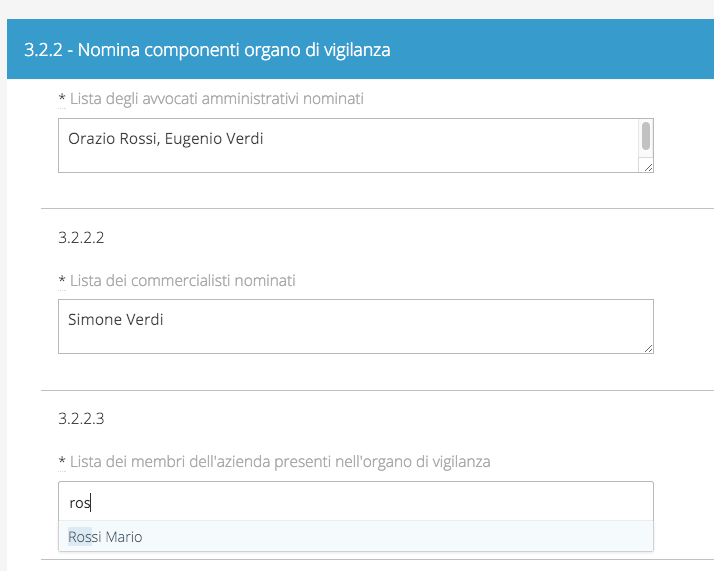
\includegraphics[width=11cm]{Pics/screen_organo_di_vigianza_con_autocompletamento.png}
			\caption{
				Schermata relativa all'inserimento di alcune informazioni in merito all'organo di vigilanza}
			\label{fig:ScreenOrganodiVigilanza}
		\end{center}
	\end{figure}
	
	Ad ogni figura di sistema è stato associato un questionario nel quale sono specificate le informazioni in merito alla carica, tra tutte la data di accettazione e scadenza dell''incarico.
	\begin{figure}[H]
		\begin{center}
			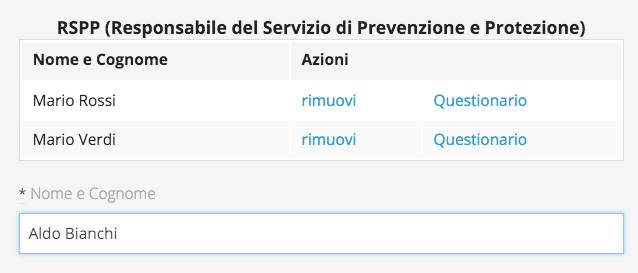
\includegraphics[width=12cm]{Pics/RemoteTrueRSPP.png}
			\caption{
				Schermata relativa all'inserimento di un RSPP.}
			\label{fig:ScreenRSPP}
		\end{center}
	\end{figure}	
	  L'associazione ad un questionario avviene generando tutte le risposte ad esso relative.\\
	  Per ogni risposta saranno preimpostati i seguenti valori:
	  \begin{itemize}
		  \item \texttt{response:} \texttt{nil};
		  \item \texttt{answerable\_type:} \texttt{"IndividualRoles"};
		  \item \texttt{answerable\_id:} codice identificativo dell'istanza specifica di \texttt{"IndividualRoles"}.
	  \end{itemize}

	Facendo Riferimento alla \autoref{fig:ScreenRSPP} e  supponendo che \textit{Aldo Bianchi} non sia attualmente presente nel database, alla pressione del tasto invio verrà generato un nuovo \textit{Individual} relativo ad \textit{Aldo Bianchi}. Successivamente verrà generato un questionario con le domande relative agli RSPP in relazione ad \textit{Aldo Bianchi}.
	
\newpage
\subsubsection{Riprogettazione della componente: \textit{DPI}}
\hl{nuova sezione}
Il termine \textit{DPI} è un acronimo di \textit{Dispositivi di Protezione Individuale}. \\
Appartengono a questa categoria tutti i dispositivi utilizzati per la prevenzione degli infortuni dei lavoratori, come ad esempio guanti, occhiali e caschetti.\\

\paragraph*{Situazione precedente alla riprogettazione} \mbox{} \\
Al momento dell'arrivo in azienda, la situazione presente era la seguente:
	\begin{figure}[H]
		\begin{center}
			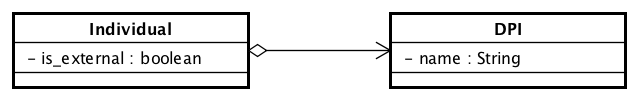
\includegraphics[width=10cm]{Pics/UMLClassiDPIversioneAllArrivo.png}
			\caption{
			Diagramma delle classi relativo ai DPI all'inizio dello stage .}
			\label{fig:UMLClassiDPIversioneAllArrivo}
		\end{center}
	\end{figure}


Come si può osservare dalla \autoref{fig:UMLClassiDPIversioneAllArrivo}, questa soluzione non impone vincoli sul nome del \gls{DPI}\G.
È necessario però segnalare se un utente non è in possesso di tutti i \gls{DPI}\G\ necessari allo svolgimento di una data mansione.\\
Questa soluzione necessitava di essere rivista poiché, non imponendo vincoli sul nome, rende impossibile gestire il caso sopracitato poiché lo stesso \gls{DPI}\G\ può essere descritto utilizzando stringhe diverse.\\
Il questionario relativo ai \gls{DPI}\G\ era stato implementato riportando tutte le domande in un unico blocco, senza differenziare le domande relative ad uno specifico \gls{DPI}\G\ da quelle generiche sui \gls{DPI}\G.

\paragraph*{Modifiche apportate}\mbox{} \\
Le modifiche hanno coinvolto sia il \gls{back-end}\G\ sia  il  \gls{front-end}\G\ dell'applicazione. \\
In particolare, nel  \gls{back-end}\G\ sono stati centralizzati i nomi dei \gls{DPI} in un unica classe. \\ 
Questa soluzione risolve il problema dell'impossibilità di riconoscimento del \gls{DPI}\G\ perché il nome è rappresentato da un riferimento ad una lista di possibili valori definiti nel pannello di amministrazione. \\
\begin{figure}[H]
	\begin{center}
		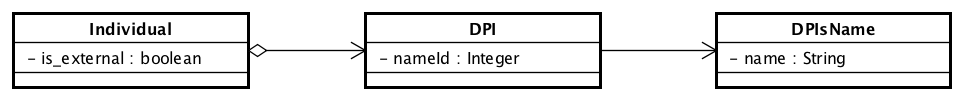
\includegraphics[width=14cm]{Pics/UMLClassiDPIRiprogettato.png}
		\caption{Diagramma delle classi relativo ai DPI dopo la riprogettazione.}
		\label{fig:UMLClassiDPIriprogettato}
	\end{center}
\end{figure}

Dopo un'attenta analisi, è stata rivista tutta l'organizzazione delle domande relative ai \gls{DPI}\G.\\
In particolare sono stati differenziate le domande relative ad uno specifico \gls{DPI}\G\ da quelle generali in merito alla gestione dei \gls{DPI}\G\ in azienda.\\
Lato \gls{front-end}\G, è stato reso possibile, per un utente amministratore, la gestione delle tipologie dei \gls{DPI}\G\ da pannello di controllo. Questo passaggio è stato reso estremamente semplice e veloce da implementare grazie all'utilizzo della gemma \hyperref[sec:ActiveAdmin]{ActiveAdmin} di Ruby on Rails.
\newpage
\begin{figure}[H]
	\begin{center}
		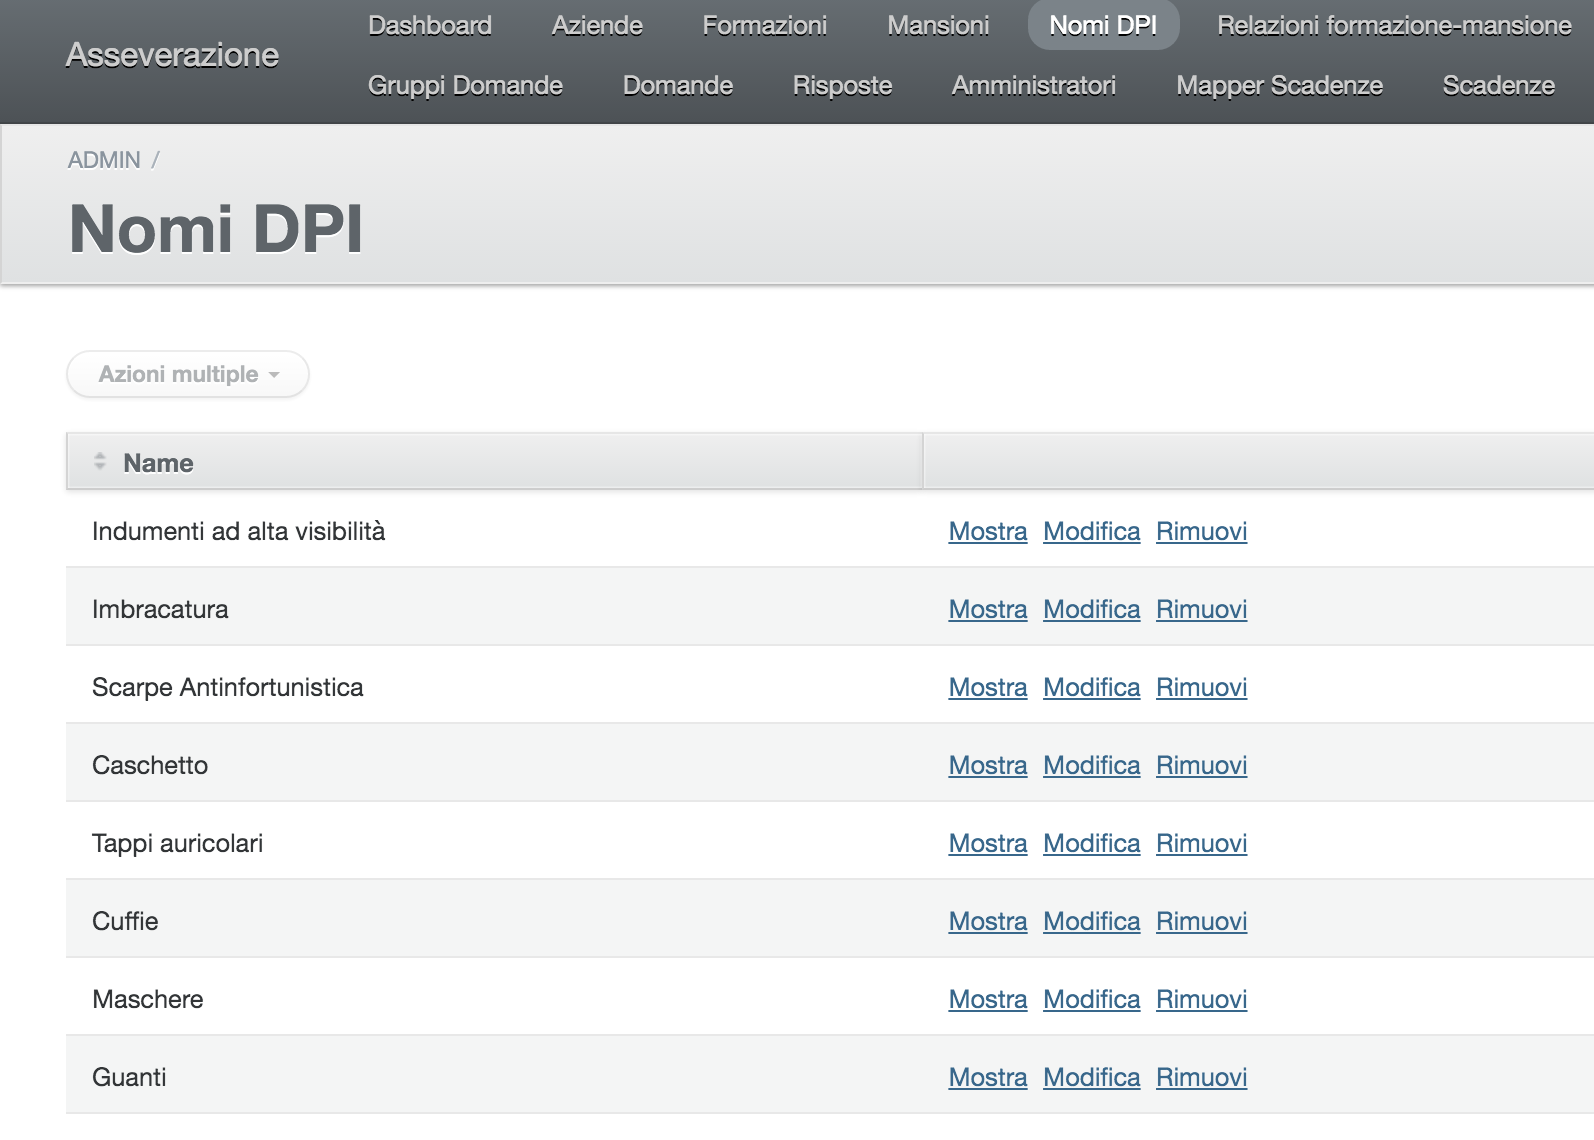
\includegraphics[width=12cm]{Pics/ActiveAdminDPI}
		\caption{Schermata relativa alla gestione dei DPI nel pannello di amministrazione.}
		\label{fig:ActiveAdminDPI}
	\end{center}
\end{figure}

E'\ stata completamente riprogettata l'interfaccia relativa alla gestione dei \gls{DPI}\G\ assegnabili ad un dipendente.\\
In particolare è stato inserito un questionario a scomparsa contenente le domande relative alla formazione obbligatoria del datore di lavoro. \\
L'input dei \gls{DPI}\G\ è stato facilitato mediante autocompletamento basato sui record della tabella \texttt{DpisName}.
\begin{figure}[H]
	\begin{center}
		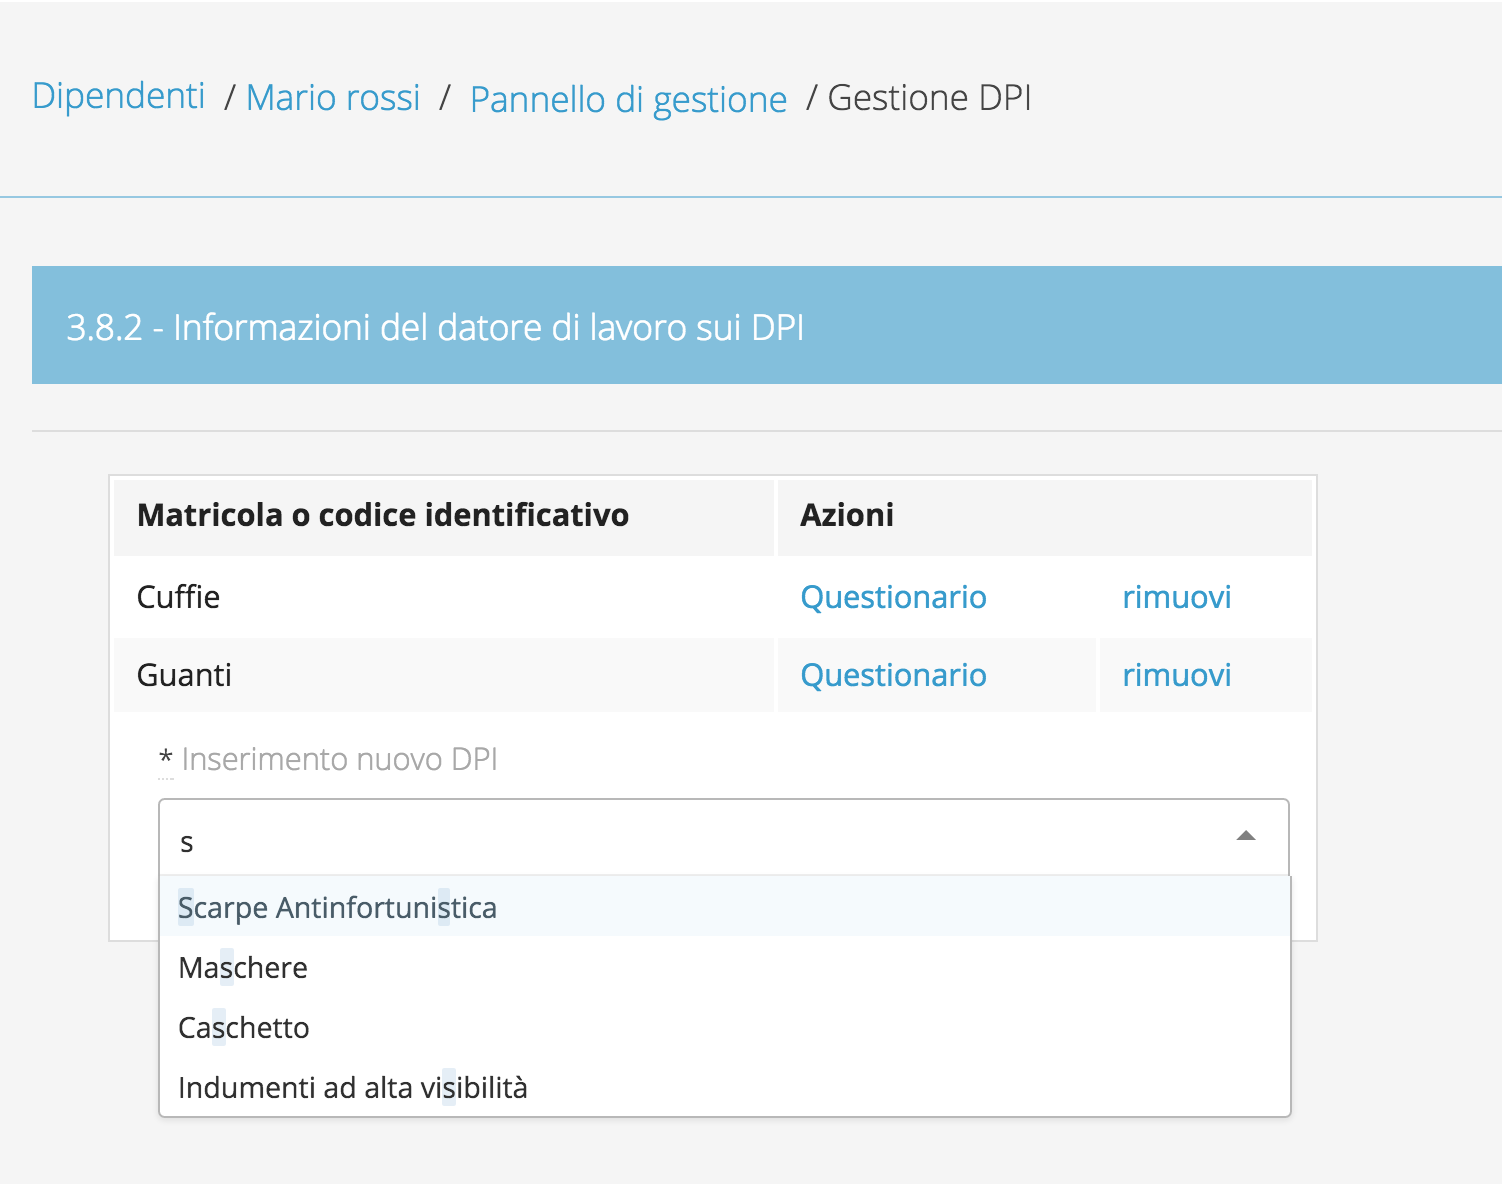
\includegraphics[width=12cm]{Pics/ScreenDPI.png}
		\caption{Schermata relativa alla gestione dei DPI nell'interfaccia utente.}
		\label{fig:ScreenDPI}
	\end{center}
\end{figure}

\newpage
\subsubsection{Riprogettazione di mansioni e formazioni}
\hl{nuova sezione}\\
Uno degli aspetti cardine del progetto è stato la gestione della relazione che intercorre tra le mansioni che svolge un dipendente e le formazioni di cui è in possesso.\\
Questa funzionalità ha richiesto una riprogettazione delle classi relative a formazioni e mansioni, oltre alla definizione delle regole relative.\\


\paragraph*{Situazione precedente alla riprogettazione} \mbox{} \\
	Al momento dell'inizio dello stage, le mansioni e le formazioni erano delle classi con una chiave esterna verso la classe \texttt{Employee} che rappresenta il dipendente in possesso di quella formazione oppure a cui è stata affidata quella mansione.\\
	Anche in questo caso, la descrizione era gestita con un campo testuale provocando ambiguità nel riconoscimento di una specifica mansione o formazione.\\
	La gestione lato \gls{front-end}\G, sebbene fosse perfettamente funzionante, risultava essere poco intuitiva.
	
\paragraph*{Modifiche apportate} \mbox{} \\
Le mansioni e le formazioni sono state riprogettate allo stesso modo dei \gls{DPI}\G, ovvero centralizzando la definizione del nome in una tabella definita allo scopo. \\
Per evitare di affaticare la lettura non verranno trattati i dettagli implementativi relativi alle singole componenti. \\
Degna di nota è invece l'integrazione tra le due componenti finalizzata alla verifica della presenza delle formazioni necessarie allo svolgimento di una mansione. \\

\begin{figure}[H]
	\begin{center}
		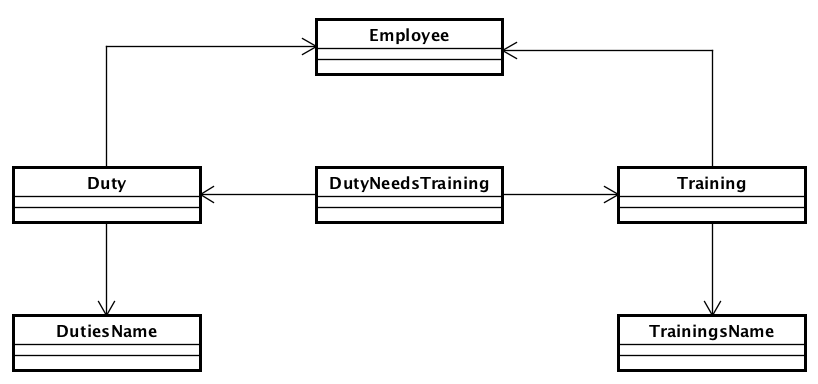
\includegraphics[width=12cm]{Pics/UMLClassiFormazioniMansioni.png}
		\caption{Diagramma delle classi di formazioni, mansioni e della relazione tra esse.}
		\label{fig:UMLClassiFormazioniMansioni.png}
	\end{center}
\end{figure}

Come è possibile osservare dalla \autoref{fig:UMLClassiFormazioniMansioni.png}, ogni record della tabella \texttt{DutyNeedsTraining} contiene un riferimento alla classe \texttt{Training} ed uno alla classe \texttt{Duty}.\\
Ogni coppia identifica una relazione che, se non soddisfatta per qualche dipendente, solleverà un allarme ad esso associato.\\
Un aspetto critico è stato dare la possibilità ad un utente amministratore di definire le regole di dipendenza tra mansioni e formazioni in modo autonomo. \\
La tabella \texttt{DutyNeedsTraining}, introdotta per mappare le dipendenze, è stata utilizzata per generare una regola relativa alla verifica della conformità tra relazioni e formazioni. La regola appena descritta è riportata nella \autoref{Drools:regolaMansioniFormazioni}.
La gestione dal pannello di controllo  stata realizzata utilizzando la gemma \hyperref[sec:ActiveAdmin]{ActiveAdmin}, rendendo  autonomo l'utilizzatore finale nella gestione delle relazioni necessità tra mansioni e formazioni.
\begin{figure}[H]
	\begin{center}
		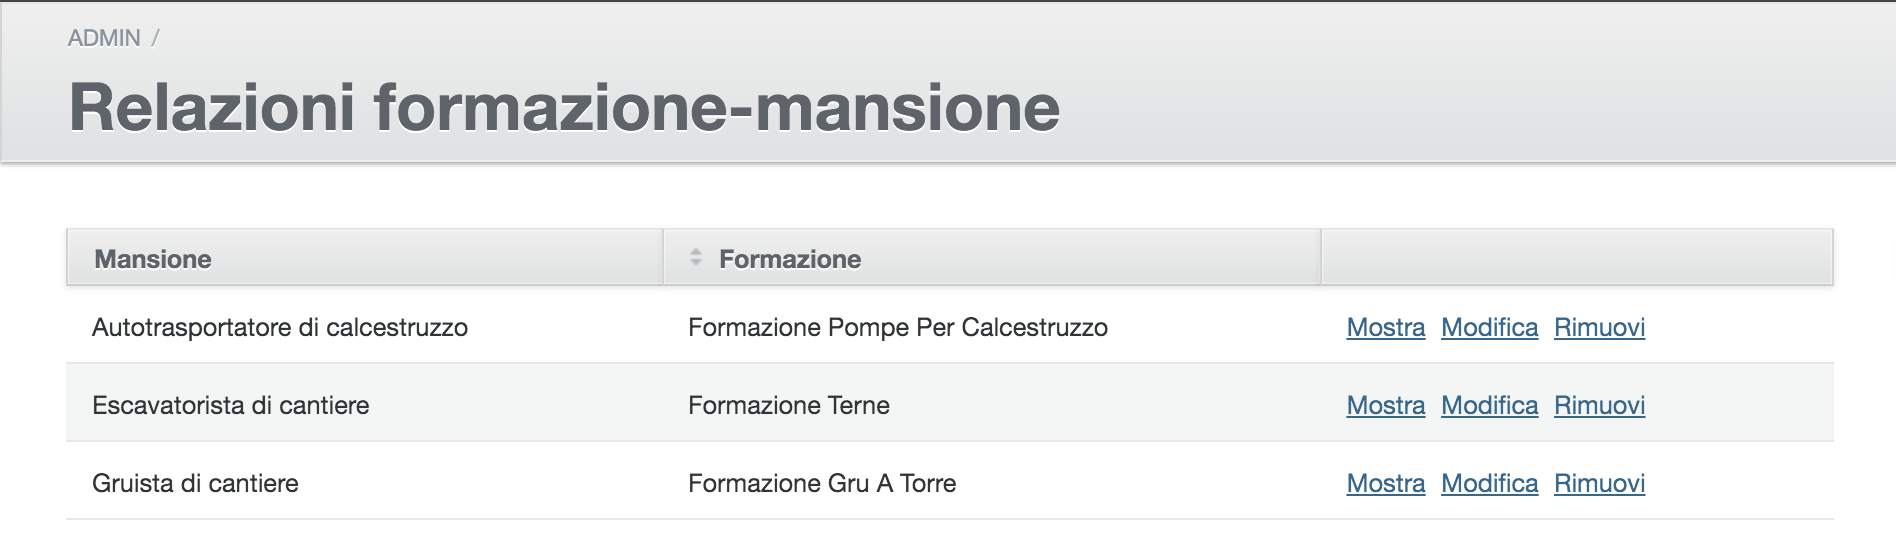
\includegraphics[width=14cm]{Pics/ScreenFormazioneMansioneAdmin.png}
		\caption{Schermata relativa alla gestione delle formazioni necessarie allo svolgimento di determinate mansioni.}
		\label{fig:ScreenFormazioneMansioneAdmin.png}
	\end{center}
\end{figure}
Per un utente autenticato, l'immissione delle mansioni e delle formazioni dei dipendenti avviene allo stesso modo dei \gls{DPI}\G. Un esempio dell'assegnazione delle mansioni è visibile in  \autoref{fig:ScreenInserimentoMansioni.png}.
\begin{figure}[H]
	\begin{center}
		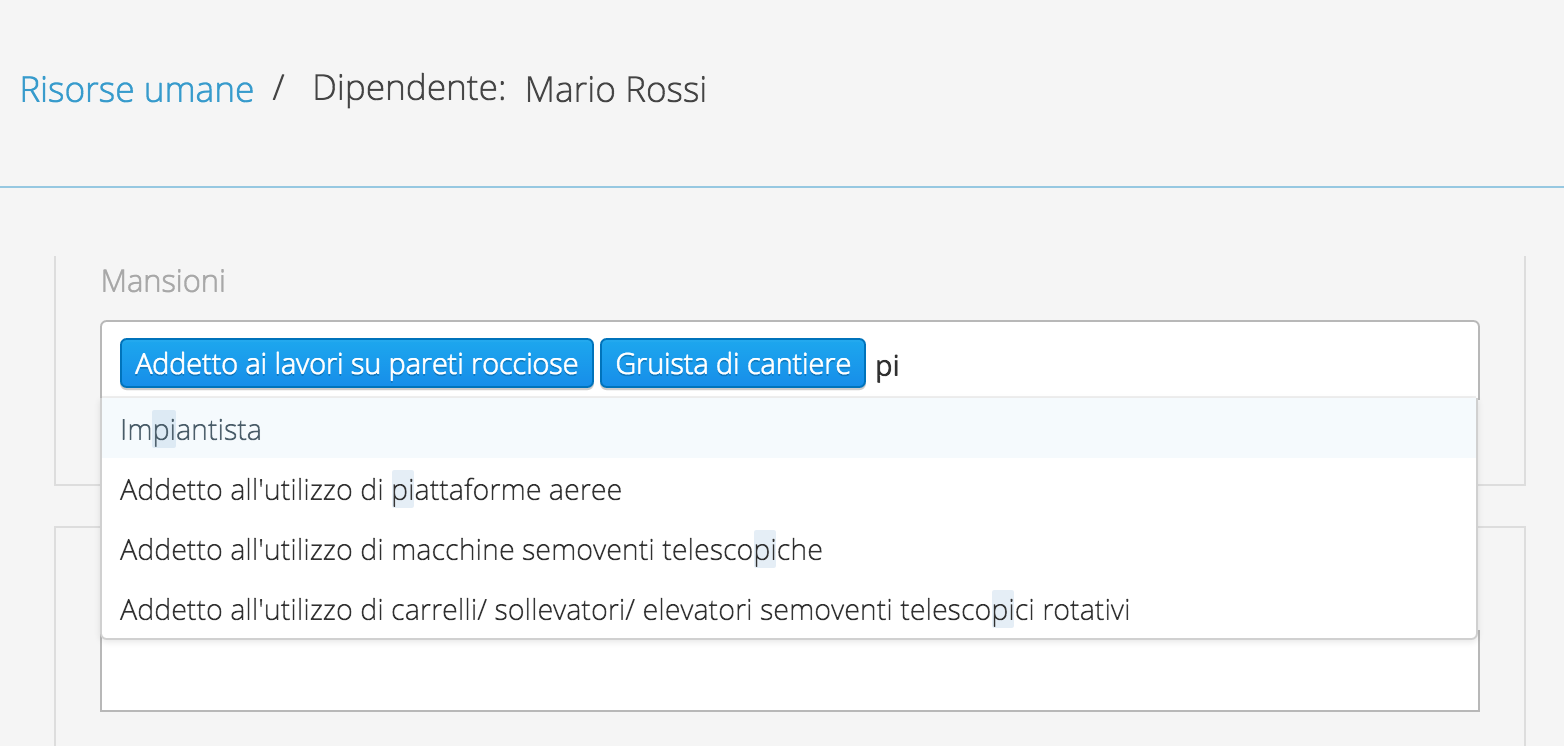
\includegraphics[width=14cm]{Pics/ScreenInserimentoMansioni.png}
		\caption{Schermata relativa all'assegnazione delle mansioni da parte di un utente autenticato.}
		\label{fig:ScreenInserimentoMansioni.png}
	\end{center}
\end{figure}
Eventuali non conformità sulle formazioni in possesso di un dipendente in relazione alla mansione che svolge saranno segnalate con un allarme. \\
 Questo approccio sposa la filosofia generale del progetto, la quale prevede che deve essere sempre possibile inserire i dati senza blocchi dettati dai vincoli di legge, in modo da evidenziare eventuali non conformità con allarmi al fine di risolverle.
\newpage
\subsubsection{Restyling della componente: \textit{Questionari}}
\hl{nuova sezione}
I questionari sono stati riprogettati solo lato \gls{front-end}\G.
Al momento dell'arrivo in azienda, le domande venivano poste in sequenza organizzate in capitoli. Questo approccio rischia di disorientare l'utente poiché al crescere del numero delle domande può trovare difficoltà nel ricordare quale sia il capitolo in questione. \\
Per ovviare a questo problema, tutte le domande sono state inserite  in un accordion e durante lo scroll il titolo viene fissato in alto . In questo modo, all'apertura della pagina sono facilmente visibili i capitoli e, durante la compilazione del questionario, il titolo del capitolo è sempre visibile.\\

\begin{figure}[H]
	\begin{center}
		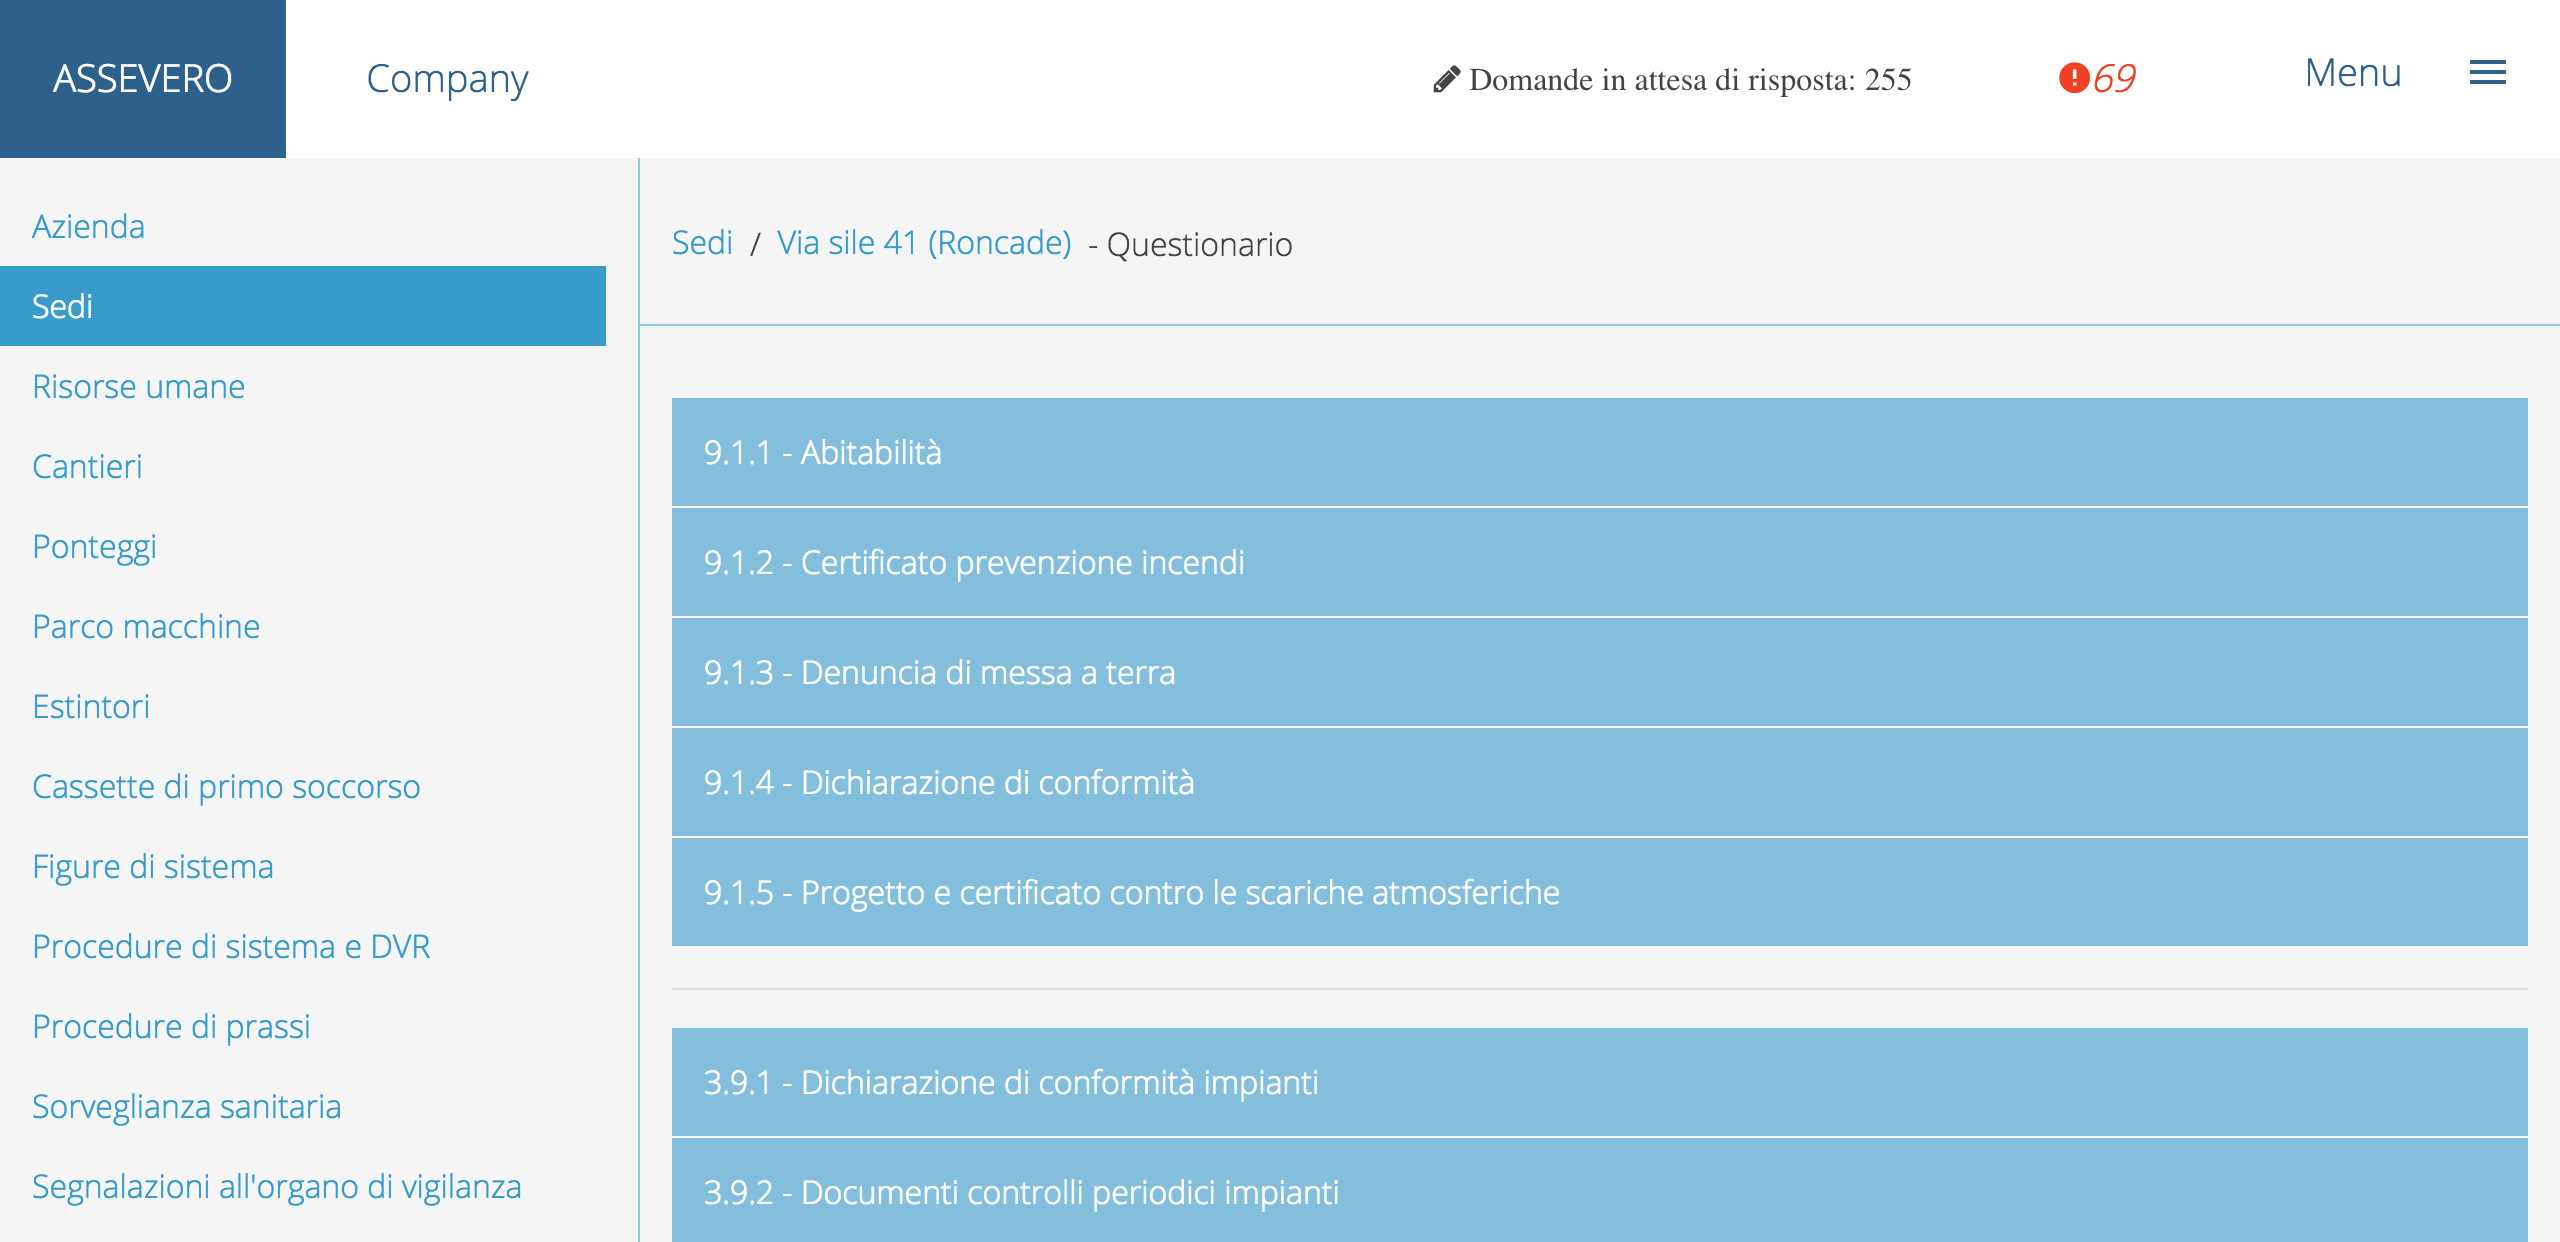
\includegraphics[width=13cm]{Pics/ScreenQuestionarioSediApertura.png}
		\caption{Schermata relativa al questionario relativo alla sicurezza nelle sedi al momento dell'apertura.}
		\label{fig:ScreenQuestionarioSediApertura.png}
	\end{center}
\end{figure}
Nella figura seguente si può notare il fatto che il titolo del capitolo rimane sempre visibile quando l'accordion è aperto.\\
\begin{figure}[H]
	\begin{center}
		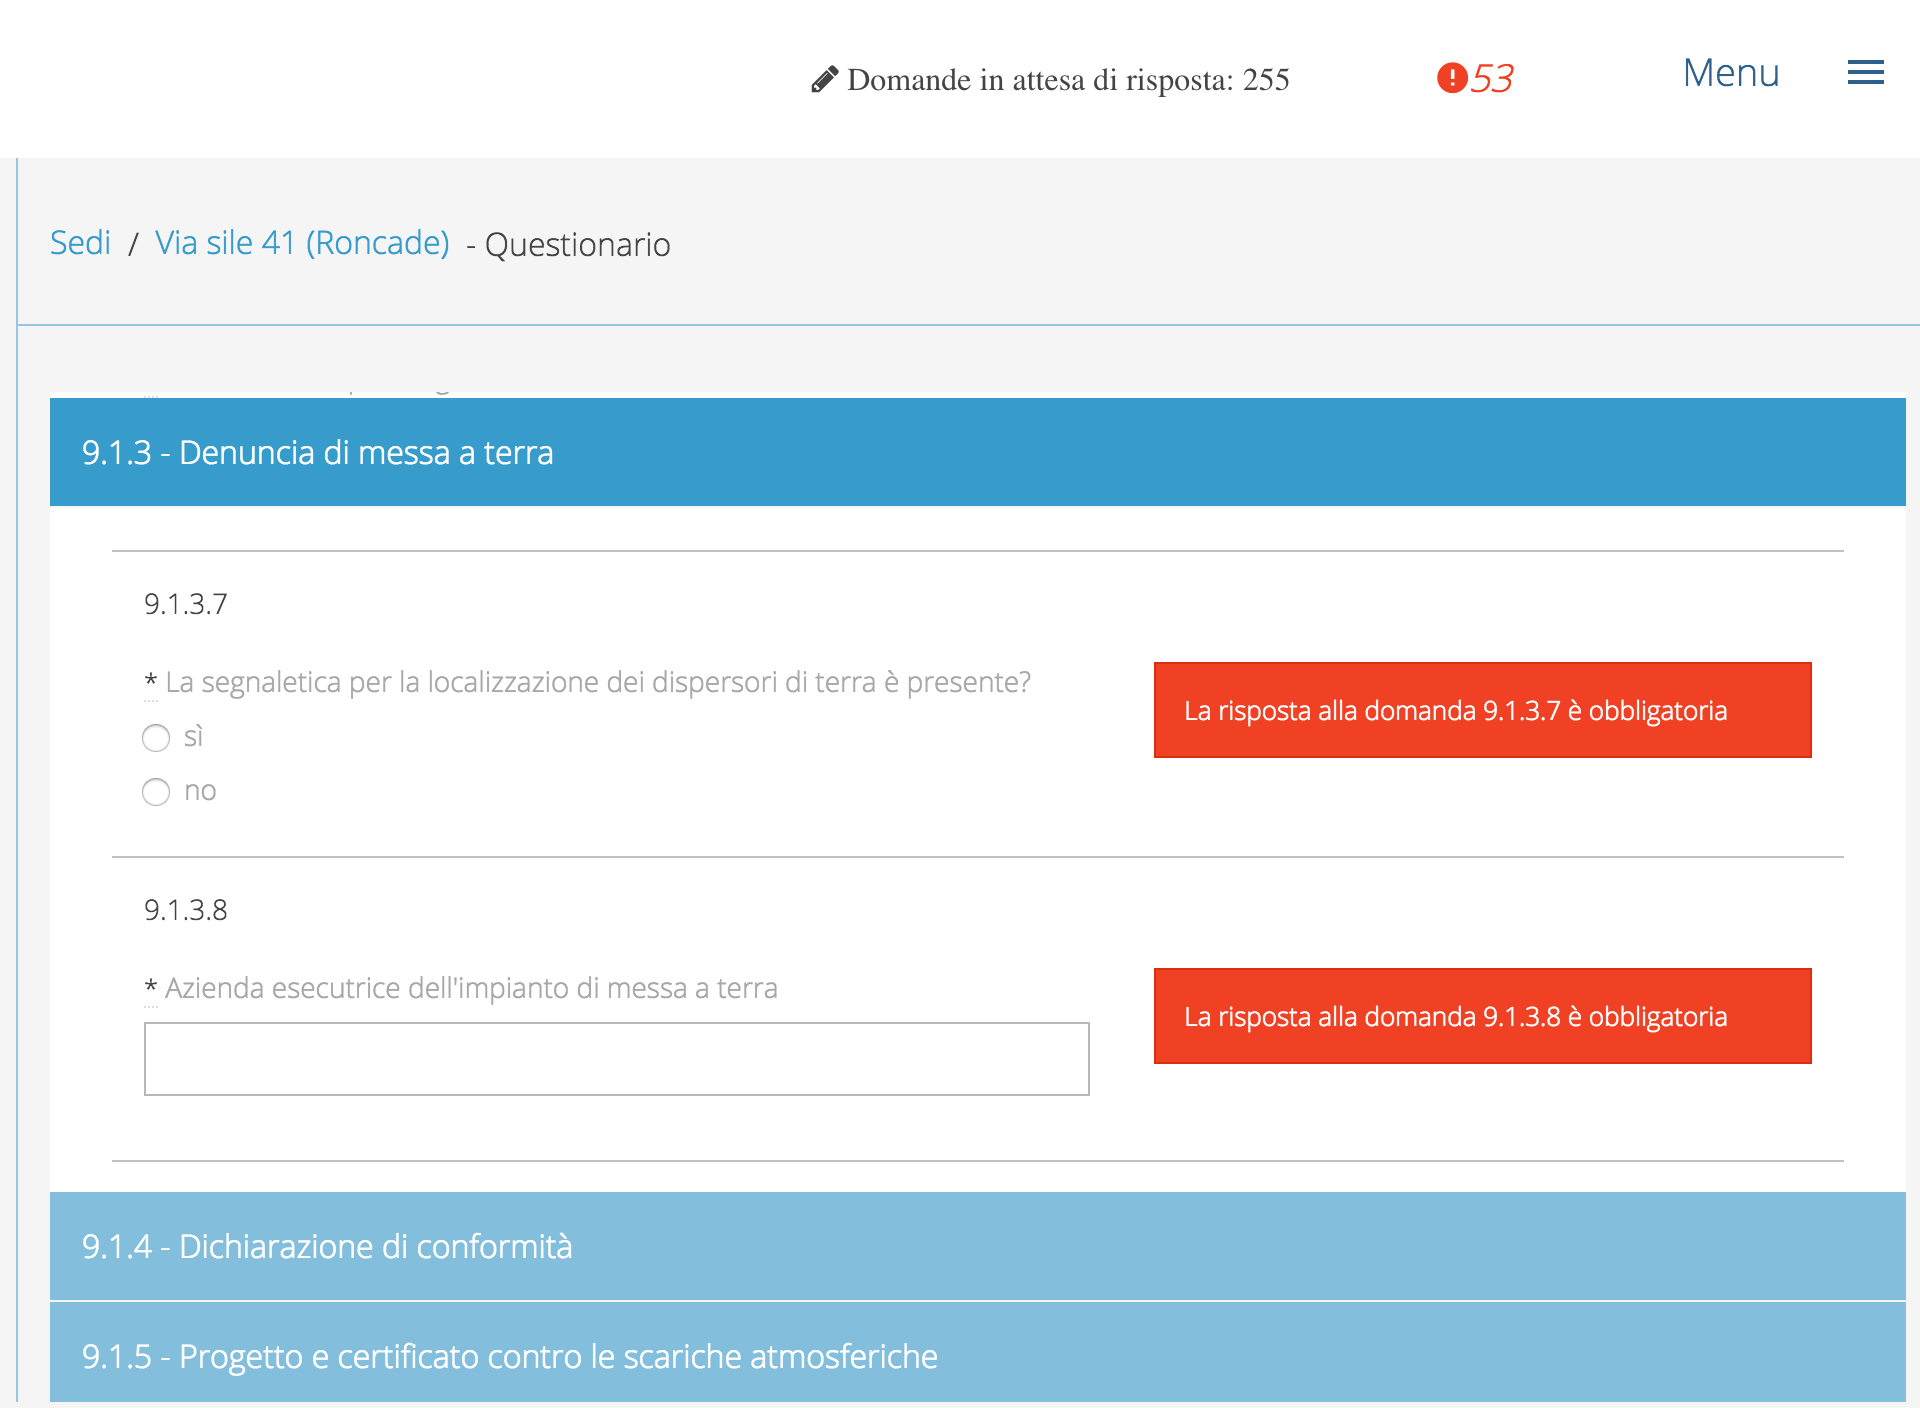
\includegraphics[width=11cm]{Pics/ScreenQuestionarioStickyHeader.png}
		\caption{Schermata relativa al questionario relativo alla sicurezza nelle sedi al momento della risposta ad una domanda.}
		\label{fig:ScreenQuestionarioStickyHeader.png}
	\end{center}
\end{figure}

 


\newpage
\subsection{Nuove componenti}
Le componenti descritte di seguito, sono state progettate e implementate nella loro interezza durante lo stage.\\

\subsubsection{\textit{Segnalazioni}}
\hl{nuova sezione}
Le segnalazioni sono delle comunicazioni inviate da un qualunque membro interno all'azienda ed indirizzate all'organo di vigilanza.\\
Le segnalazioni hanno lo scopo di sollevare il responsabile dalle responsabilità derivanti da violazioni avvenute sotto la sua supervisione. \\
Le comunicazioni all'organo di vigilanza infatti, non possono essere anonime e demandano ufficialmente la responsabilità delle eventuali violazioni a tale organo il quale dovrà decidere per eventuali azioni correttive.
	
	\paragraph*{Progettazione}\mbox{} \\
	Come è possibile osservare dalla \autoref{fig:UMLClassiSegnalazioni}, le segnalazioni sono state implementate come una classe (\texttt{Report}) con una chiave esterna verso la classe \texttt{Individual}. \\
	La presenza del riferimento verso un'istanza della classe \texttt{Individual} è obbligatoria, soddisfacendo quindi il vincolo di non anonimato delle segnalazioni.\\
	\begin{figure}[H]
		\begin{center}
			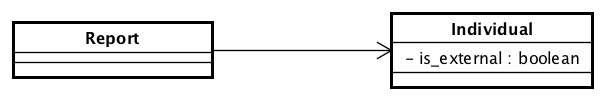
\includegraphics[width=12cm]{Pics/UMLClassiSegnalazioni.png}
			\caption{Diagramma delle classi relativo alle segnalazioni.}
			\label{fig:UMLClassiSegnalazioni}
		\end{center}
	\end{figure}
	Specifiche direttive del committente hanno richiesto l'inserimento di tre date rilevanti al fine della gestione delle segnalazioni:
	\begin{itemize}
		\item \textit{Data di invio della segnalazione all'alta direzione;}
		\item \textit{Data di invio della segnalazione dall'alta direzione all'organo di vigilanza;}
		\item \textit{Data di invio della risposta alla segnalazione da parte dell'organo di vigilanza al soggetto interessato.}
	\end{itemize}
	In accordo con la filosofia del progetto, sono state gestite la presenza e sequenzialità delle date con degli allarmi in caso di errato inserimento.\\
	Per facilitare la gestione delle segnalazioni, nell'interfaccia utente relativa ad esse sono riportate tutte le date. Questo approccio permette di tenere sempre traccia dello stato delle segnalazioni ed agevola la verifica da parte delle autorità competenti.\\
	Uno sviluppo futuro, prevede l'archiviazione delle segnalazioni le quali hanno data di invio della risposta alla segnalazione da parte dell'organo di vigilanza al soggetto interessato più vecchia di 30 giorni. Questa soluzione è stata progettata, ma non implementata nel periodo di stage a causa dell'esaurimento del monte ore disponibile.
	\begin{figure}[H]
		\begin{center}
			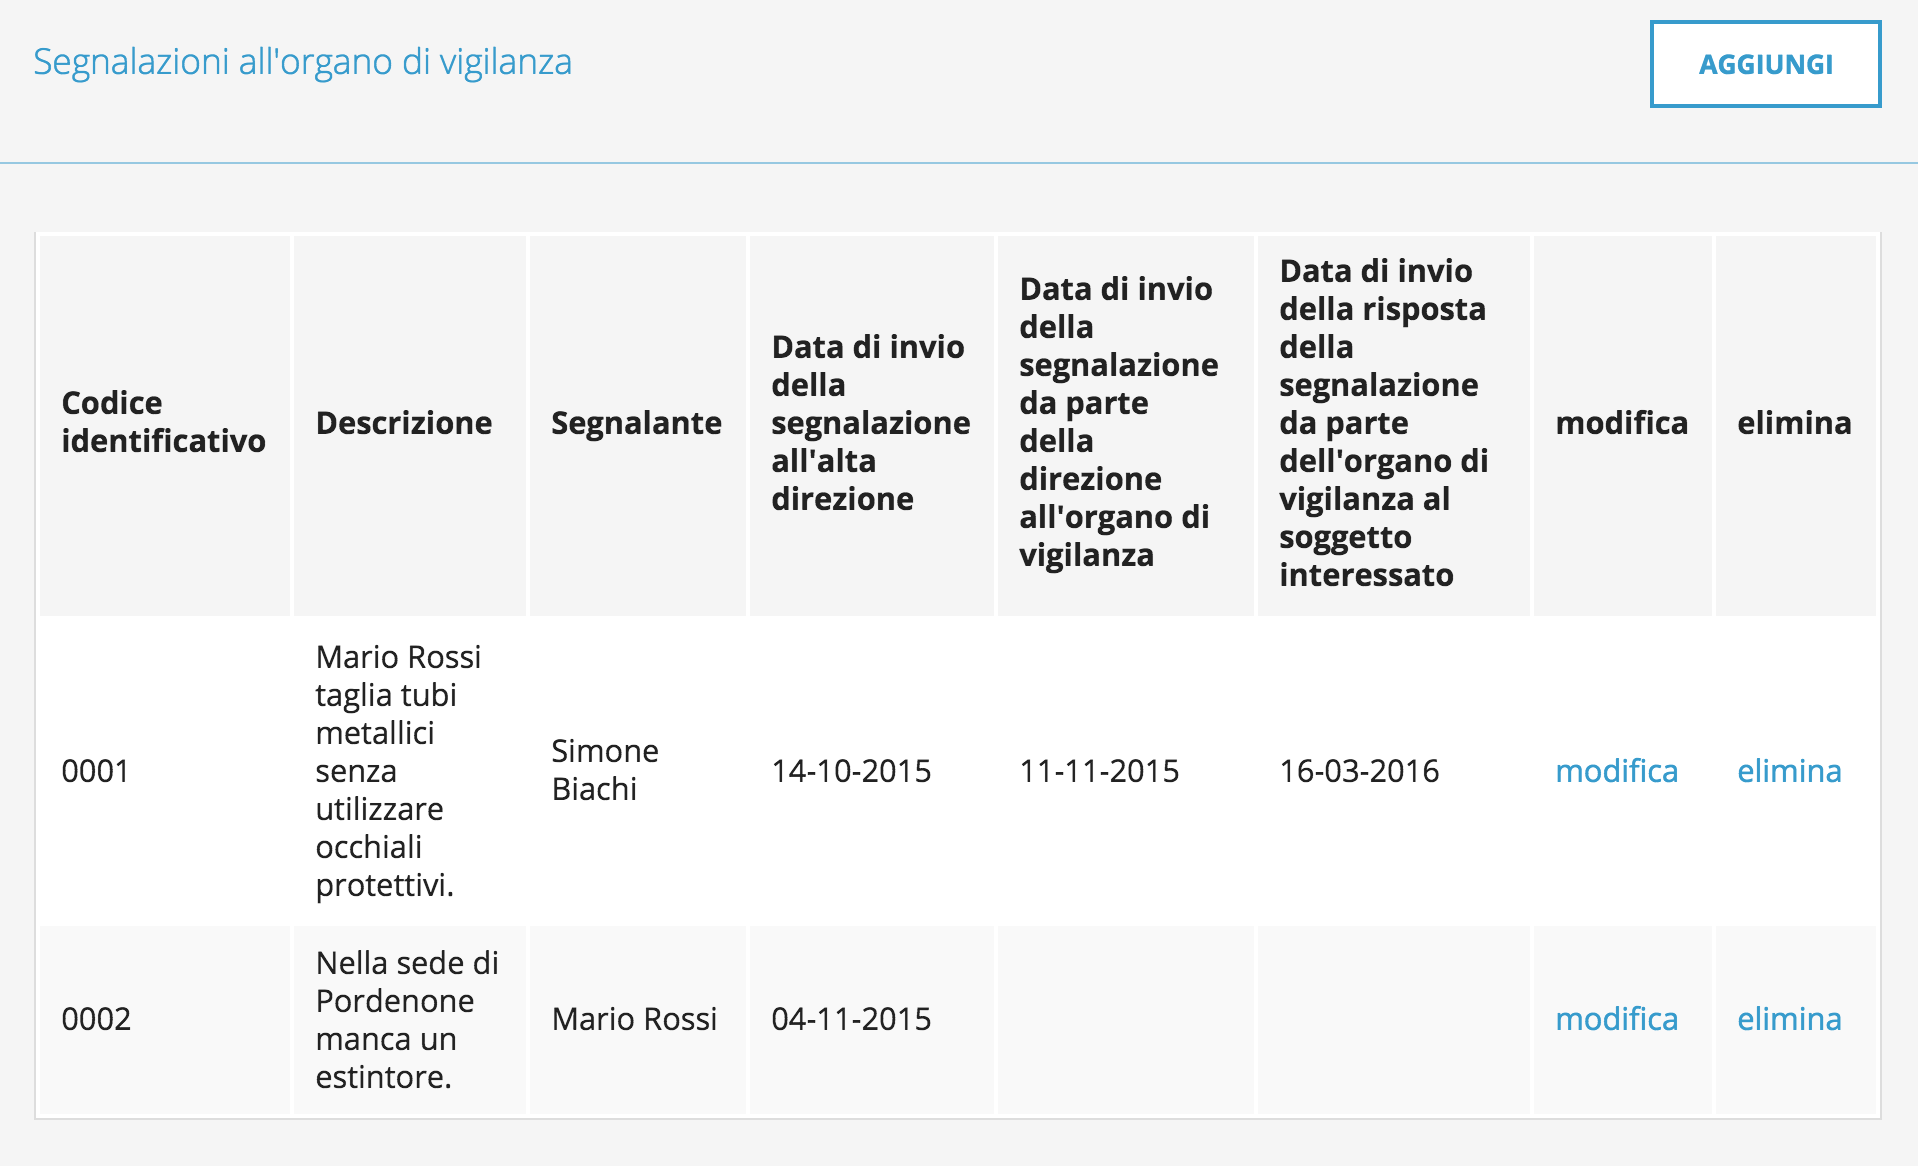
\includegraphics[width=12cm]{Pics/ScreenSegnalazioni.png}
			\caption{Schermata relativa alla gestione delle segnalazioni.}
			\label{fig:ScreenSegnalazioni}
		\end{center}
	\end{figure}
\newpage
\subsubsection{\textit{Procedure}}
\hl{Nuova sezione}\\
	Le procedure si distinguono in due categorie distinte:
	\begin{itemize}
		\item \textit{Procedure di prassi:}	\\
			Procedure derivanti da uno studio eseguito dall'\gls{INAIL}\G\ sulla base dell'analisi degli infortuni sul lavoro avvenuti nel tempo.
		\item \textit{Procedure di sistema:}\\
			Procedure proprie dell'azienda. La loro composizione compone il  \gls{DVR} (Documento di Valutazione dei Rischi).
	\end{itemize}

	\paragraph*{Progettazione}\mbox{}\\
		\subparagraph*{Procedure di prassi}\mbox{}\\
		Queste procedure sono state fornite come collezione di domande. È risultato naturale quindi gestirle mediante dei questionari.\\
		Dopo un'attenta analisi delle domande, sono stati individuati sette filoni principali che sono stati usati per spezzare un questionario composto di 189 domande.\\
		Ad ognuno di questi è associato un questionario come è possibile osservare nella \autoref{fig:ScreenProcedureDiPrassi}.
		
		\begin{figure}[H]
			\begin{center}
				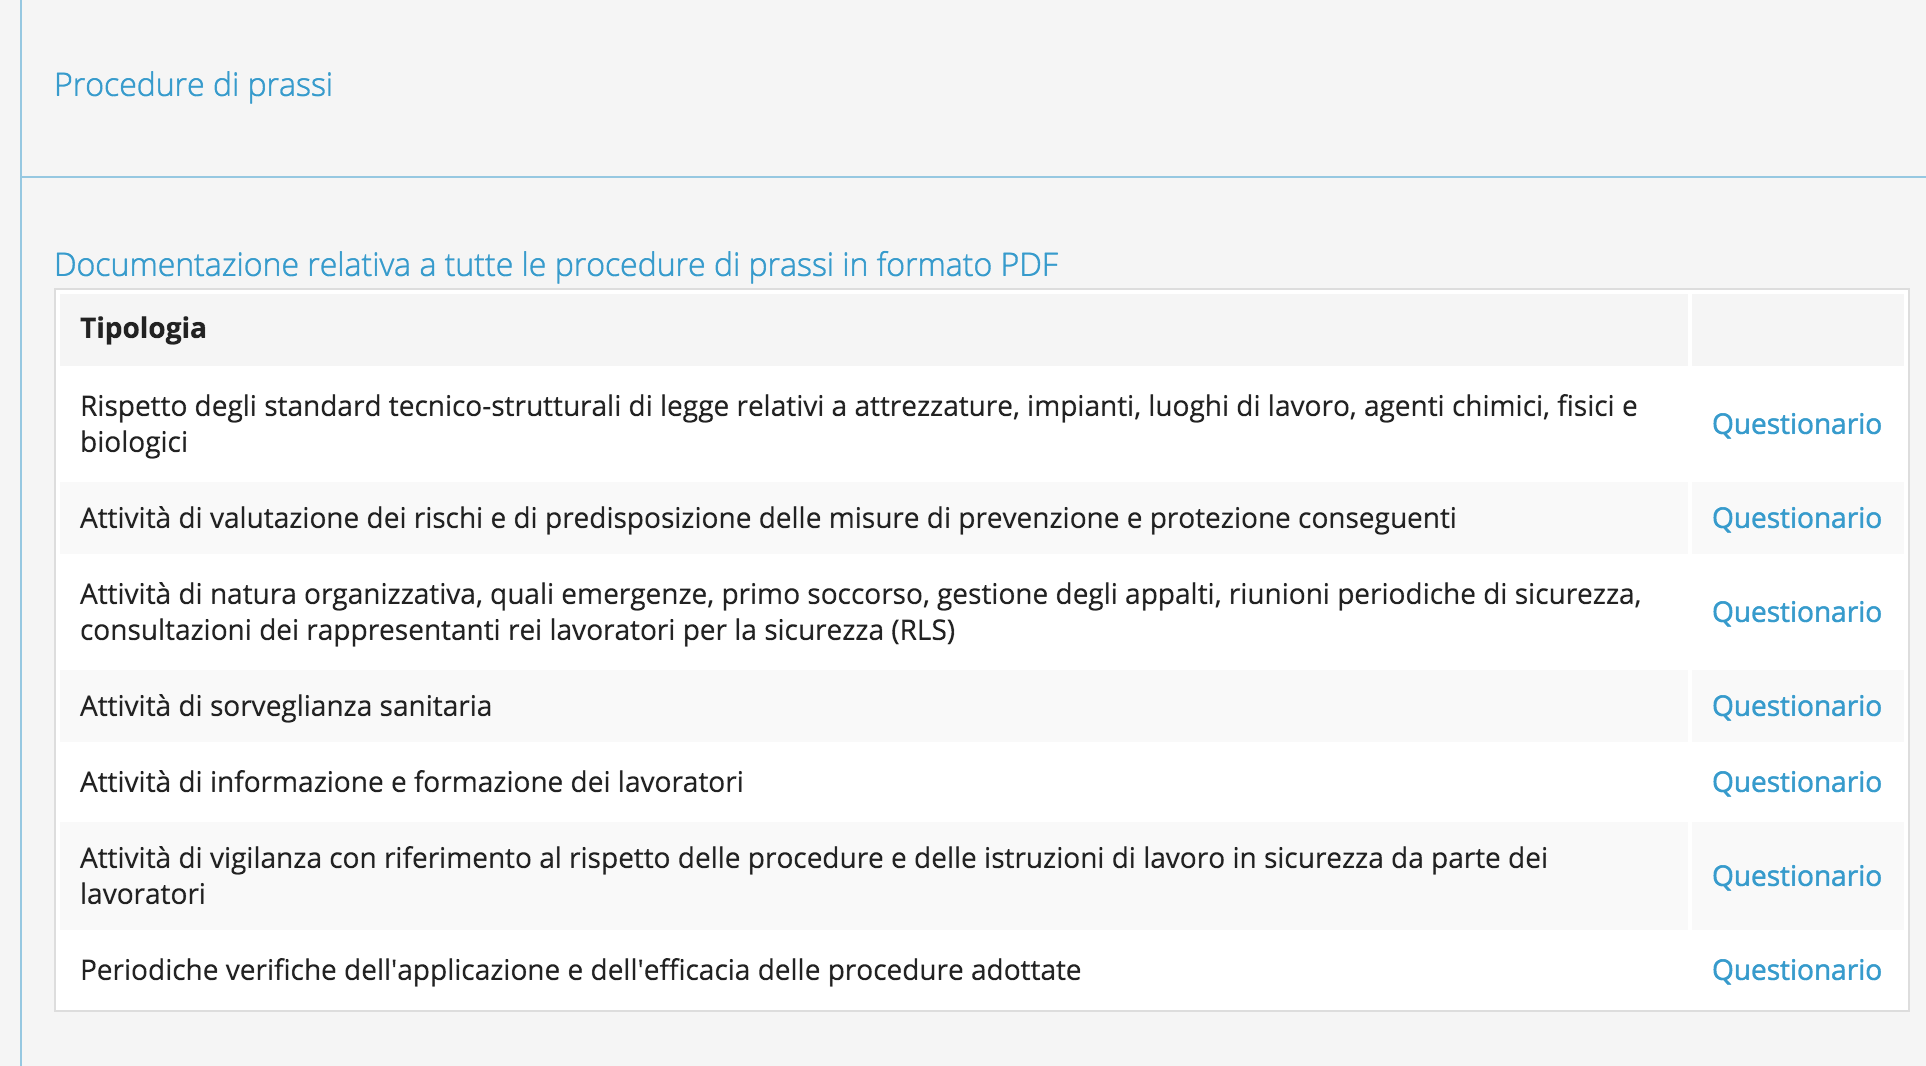
\includegraphics[width=14cm]{Pics/ScreenProcedureDiPrassi.png}
				\caption{Schermata relativa alla gestione delle procedure di prassi.}
				\label{fig:ScreenProcedureDiPrassi}
			\end{center}
		\end{figure}
		Per avere un quadro generale della conformità dell'azienda rispetto alle procedure di prassi è stata implementata l'esportazione di tutte le domande in un unico documento in formato PDF.
		
		\subparagraph*{Procedure di sistema}\mbox{}\\
			
			Le procedure di sistema sono state implementate mediante un apposito modello \texttt{Procedure} direttamente collegato a \texttt{Company}. Sono state inserite le informazioni relative alle revisioni di ogni procedura.\\
			Come è possibile osservare dalla \autoref{fig:ScreenDVR}, sono state inserite le domande relative al \gls{DVR}\G\ nell'interfaccia utente con un questionario a scomparsa.
			
			\begin{figure}[H]
				\begin{center}
					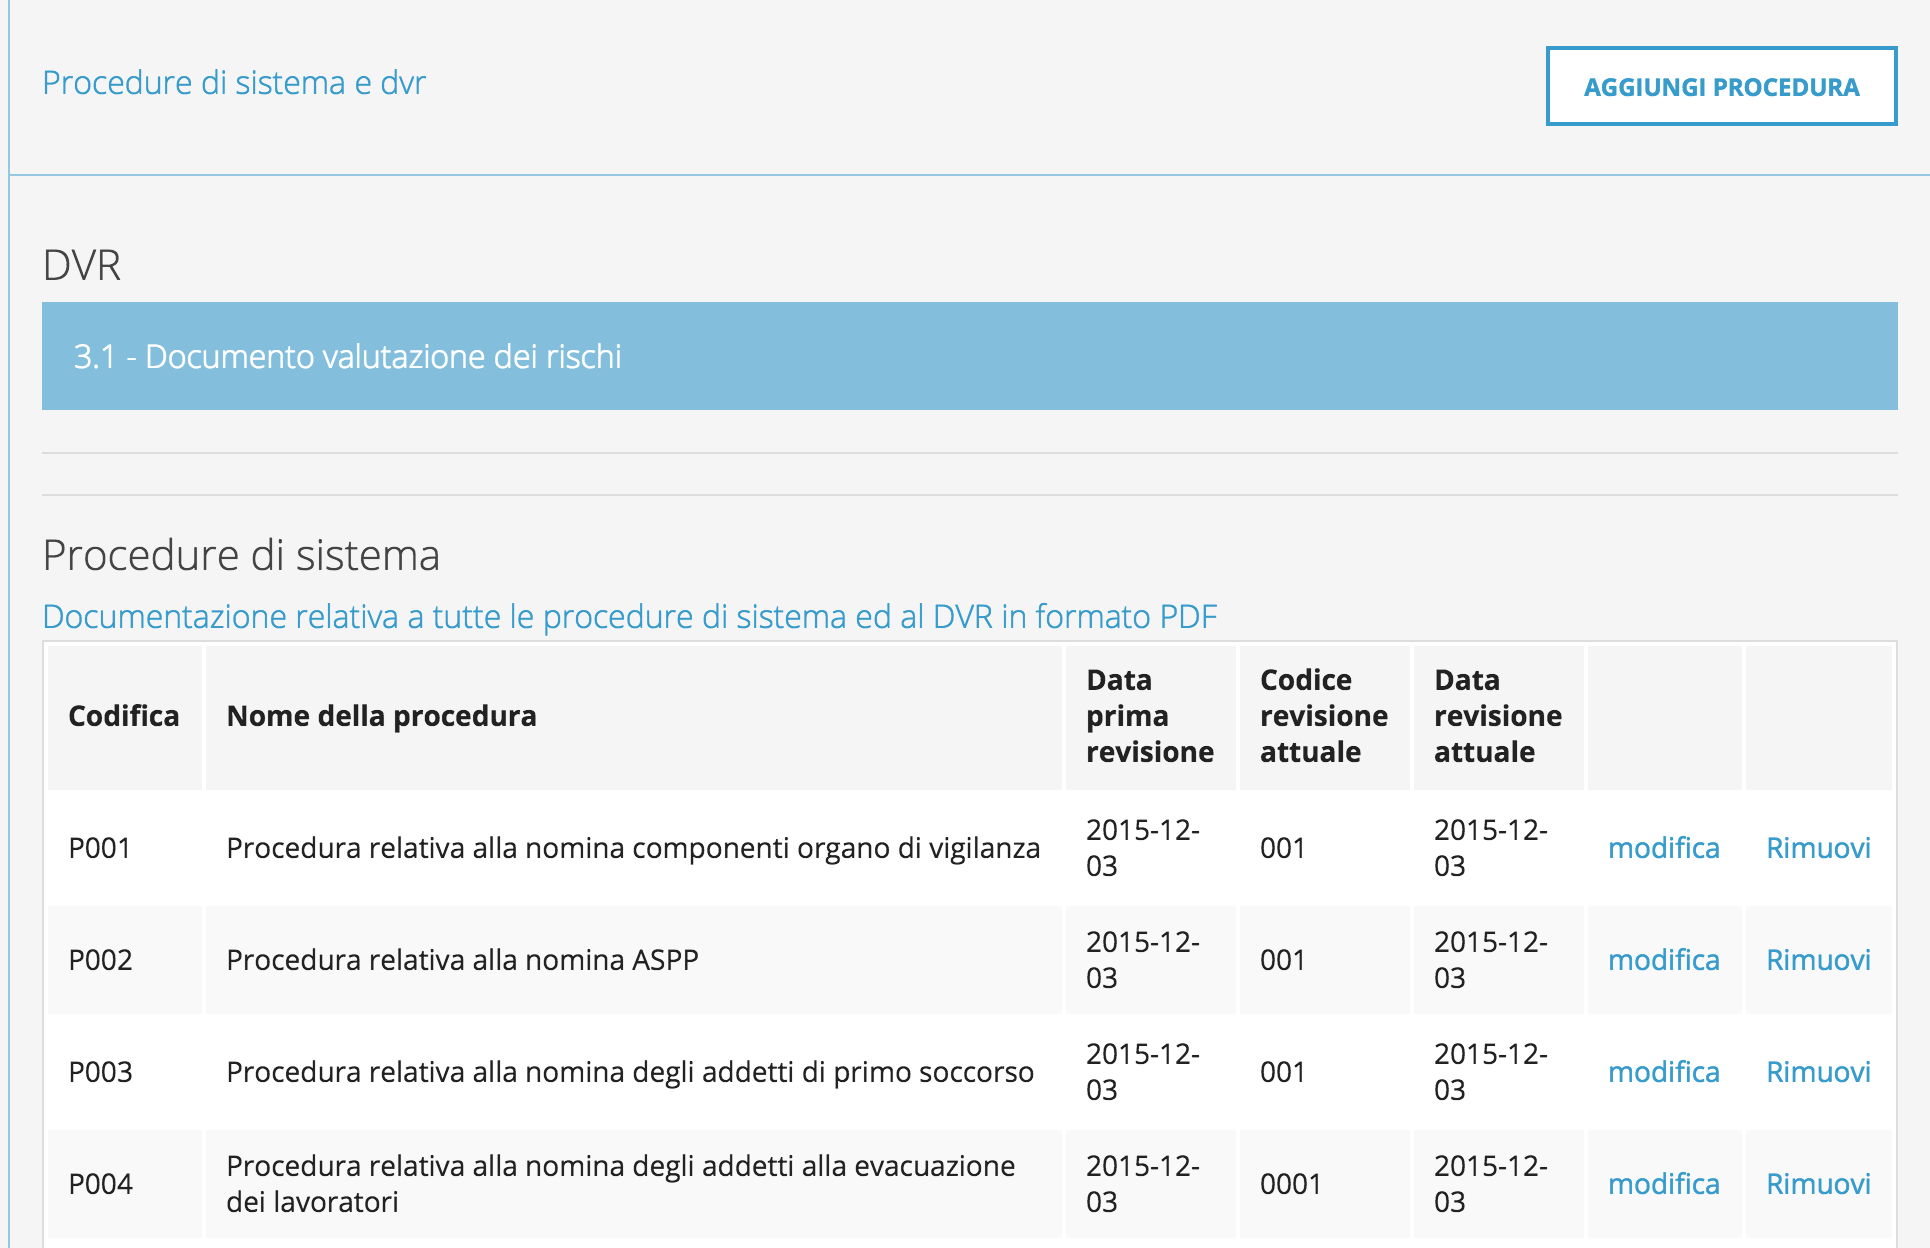
\includegraphics[width=14cm]{Pics/ScreenDVR.png}
					\caption{Schermata relativa alla gestione delle procedure di sistema.}
					\label{fig:ScreenDVR}
				\end{center}
			\end{figure}
			Per mettere a disposizione un quadro generale delle procedure di sistema è stata implementata l'esportazione di tutte le domande in un unico documento in formato PDF.

	\paragraph*{Criticità incontrate}\mbox{}\\
		Per mantenere una coerenza logica, tutti gli aspetti inerenti le procedure sono state gestite con un singolo controller.\\
		Questo ha subito evidenziato numerose criticità in quanto è stato necessario realizzare due index, ma l'URL \texttt{\textbackslash procedures} può corrispondere ad una sola azione (\texttt{index}).\\
		È stato necessario creare delle apposite rotte per permettere di raggiungere entrambe le risorse.
		%più controller e viste associate allo stessa categoria, uno ha il modello l'altro il questionario
\newpage
\subsubsection{\textit{Dispositivi di protezione collettivi}}
\hl{nuova sezione}\\
La gestione dei \gls{DPC}\G\ richiede di tenere traccia delle informazioni relative al loro posizionamento. \\
In particolare sono stati gestiti Estintori e cassette di primo soccorso. \\
Le immagini \autoref{fig:ScreenIndexEstintori} e \autoref{fig:ScreenRemoteTrueEstintori}, arrecano esempi relativi agli estintori, ma la trattazione dei due modelli è analoga. La differenza è individuabile solo nella gestione della scadenza che per gli estintori è unica, mentre per le cassette di primo soccorso chiede di memorizzare quella dei due componenti più vicini alla data di scadenza.

\paragraph*{Progettazione}\mbox{}\\
La soluzione individuata prevede la creazione di una associazione con l'interfaccia \textit{Locationable} come è possibile osservare dalla \autoref{fig:UMLClassiDPC}.\\
Questo approccio è proprio di Ruby on Rails e permette di riferire un oggetto specificandone il nome della classe e l'id a patto che la classe interessata dichiari di essere essere un \textit{Locationable}.\\
Nel caso di specie, le classi che dichiarano di essere raggiungibili mediante l'interfaccia \textit{Locationable} sono\texttt{Location} e \texttt{ConstructionSite}, permettendo quindi di assegnare \gls{DPC}\G\ a sedi e cantieri.
\begin{figure}[H]
	\begin{center}
		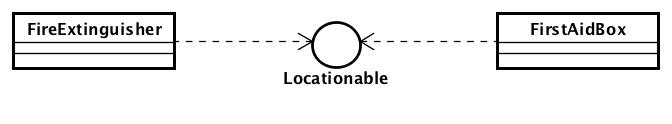
\includegraphics[width=12cm]{Pics/UMLClassiDPC.png}
		\caption{Diagramma delle classi relativo ai \gls{DPC}\G.}
		\label{fig:UMLClassiDPC}
	\end{center}
\end{figure}

Al momento dell'assegnazione dei \gls{DPC}\G\ ad una sede oppure ad un cantiere, sono stati resi selezionabili solamente quelli che non risultano essere impegnati in altri luoghi.\\
È stata implementata una pagina nella quale sono visibili tutti gli estintori (e rispettivamente per le cassette di primo soccorso) nella quale è indicata la loro allocazione al fine di facilitare la localizzazione agevolando le operazioni di manutenzione.

\begin{figure}[H]
	\begin{center}
		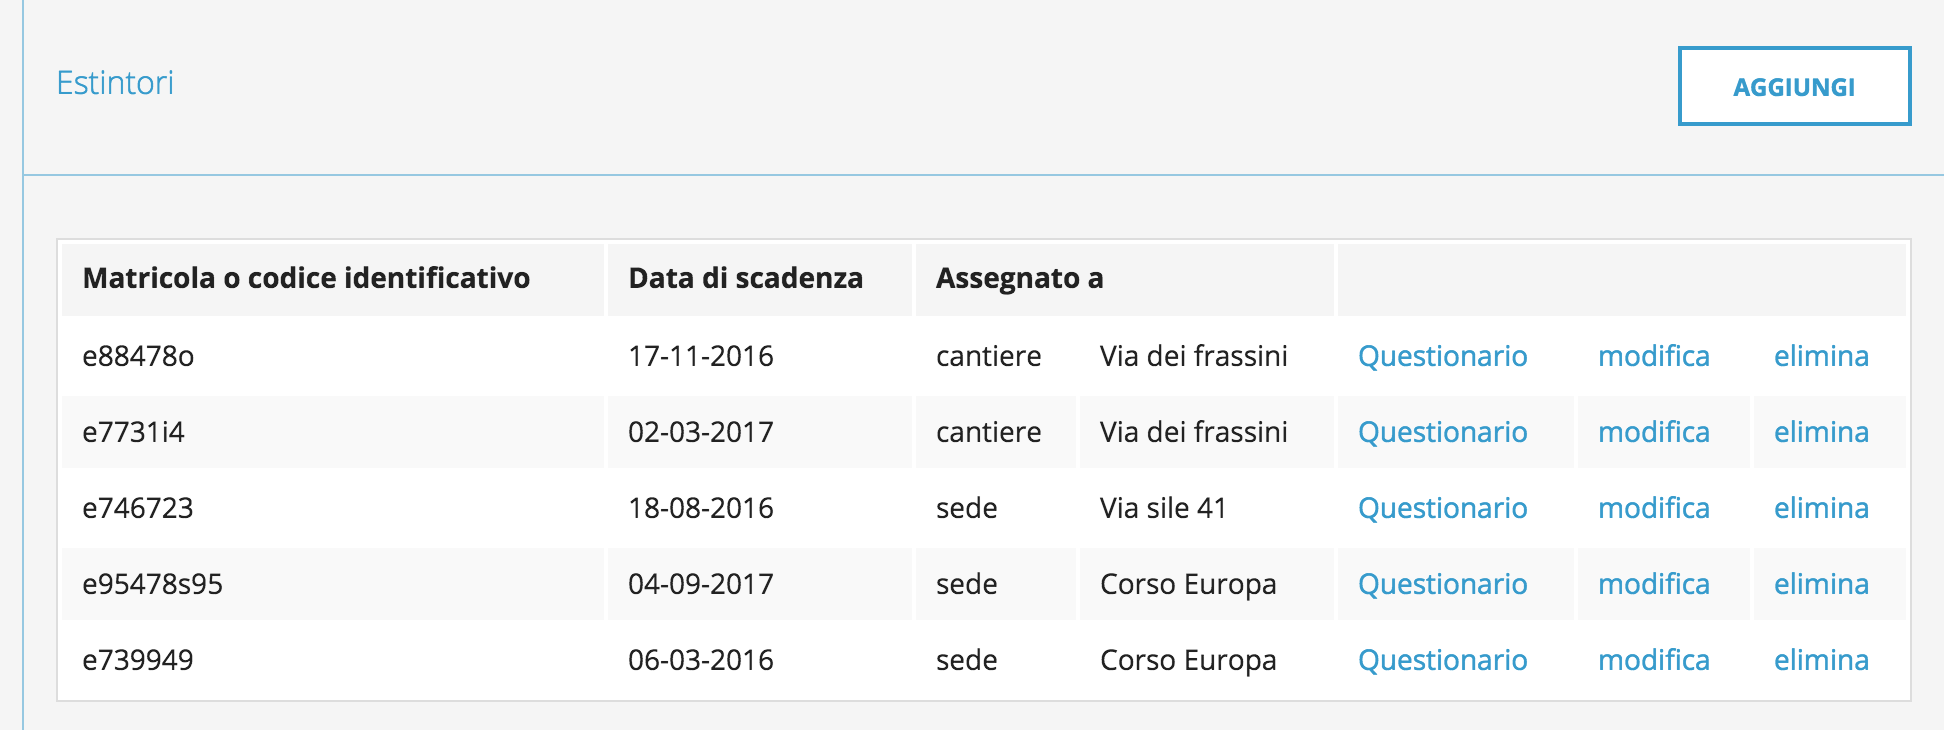
\includegraphics[width=15cm]{Pics/ScreenIndexEstintori.png}
		\caption{Schermata relativa agli Estintori in azienda.}
		\label{fig:ScreenIndexEstintori}
	\end{center}
\end{figure}




	\paragraph*{Criticità incontrate}\mbox{}\\
	Al fine di rendere agevole ed intuitiva la gestione dei \gls{DPC}\G, è stato creato un meccanismo di gestione dinamica mediante chiamate \gls{Ajax}\G. \\
	Fare ciò è stato necessario introdurre un nuovo tipo di file di template di Rails(\textit{*.js.erb}) e strutturare i template \textit{*.html.erb} in modo tale da essere compatibili con il nuovo pattern mediante invocazioni remote.\\
	Questo tipo di attività, essendo molto verbosa e delicata nella gestione, ha richiesto più tempo rispetto a quanto pianificato.
		%remote true
		\begin{figure}[H]
			\begin{center}
				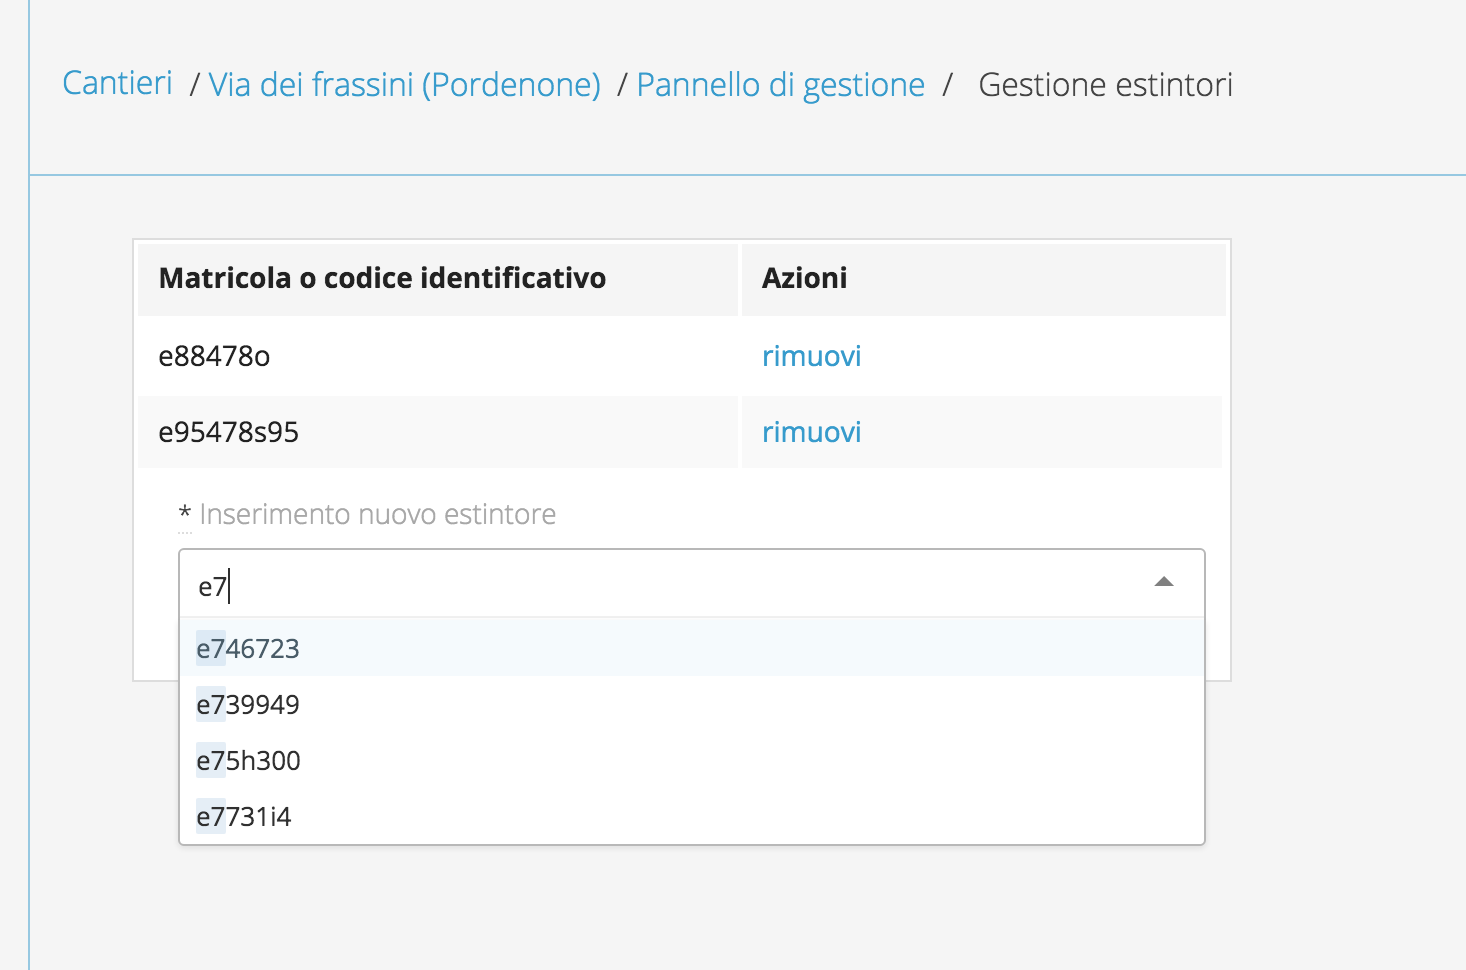
\includegraphics[width=12cm]{Pics/ScreenRemoteTrueEstintori.png}
				\caption{Schermata relativa alla dotazione di estintori in un luogo .}
				\label{fig:ScreenRemoteTrueEstintori}
			\end{center}
		\end{figure}
		

\newpage
\subsection{Regole Drools}
\hl{nuova sezione}
\label{Drools:regole}
\hl{In questa sezione vengono riportate alcune tra le regole Drools più significative.}
\subsubsection{Riconoscimento di un indoviduo che ricopre una mansione per la quale non è formato}
	\label{Drools:regolaMansioniFormazioni}
	\begin{verbatim}
	rule "Individuo ricopre una mansione per la quale non è formato"
	when
	$t: Training()
	$d: Duty(trainings contains $t)
	$i: Individual(duties contains $d, trainings not contains $t)
	then
	System.out.println($i.getFirstName() + ' ' + $i.getLastName() + "ha la mansione" +
	$d.getName() + " ma non la formazione " + $t.getName() );
	end
	\end{verbatim}
	\begin{itemize}
		\item \$t filtro sulle formazioni;
		\item \$d filtro sulle mansioni che necessitano della formazione \$t;
		\item \$i filtro su tutti gli individui che svolgono la mansione \$d ma non sono in possesso della formazione \$t.
	\end{itemize}
	Le corrispondenze di questa regola sono tutti gli individui individui che svolgono una qualunque mansione per la quale non sono correttamente formati.\\
	Al verificarsi di queste condizioni, viene generato un allarme il cui contenuto è specificato dalla stampa disposta dalla \gls{RHS}\G.
	
\subsubsection{Mancanza del CPI per sedi con superficie maggiore di trecento metri quadri}
\label{Drools:regolaCPISuperficie}

	\begin{verbatim}
		rule "CPI assente e superficie e la superficie della sede è  maggiore di 300 metri quadri"
		when
		$s: 	  Location(surfaceArea > 300)
		$a: 	  Answer(answerableType == "Location", answerableId == $s.getId(), 
					questionCode == "location_needs_CPI", response == "no")
		then
					System.out.println("La sede all\'indirizzo"+ $s.getAddress() +
					 ", ha una superficie maggiore di 300 metri quadri, richiede quindi il CPI. ");
		end
	\end{verbatim}

	\begin{itemize}
		\item \$s filtro sulle sedi;
		\item \$a filtro sulle risposte riferite alla sede \$s relative alla presenza del \gls{CPI}\G;
	\end{itemize}
	Le corrispondenze di questa regola sono tutte le risposte alle domande con risposta negativa relative alla presenza del CPI (Certificato Prevenzione Incendi) nelle sedi con più di trecento metri quadri di superficie.

\newpage
\section{Verifica e validazione}
	\hl{nuova sezione}	
	Al termine della fase di sviluppo di ogni modulo del progetto, si è proceduto con l'attività di verifica, per assicurarsi che il prodotto fosse privo di bug e conforme ai requisiti.\\
	Il codice relativo ai modelli prodotto durante lo stage è stato sottoposto a test d'unità man mano che veniva implementato. Dal punto di vista implementativo, i test sono stati realizzati utilizzando la gemma \textit{Minitest} di Ruby on Rails.\\
	Nel caso delle segnalazioni, è stato utilizzato l'approccio \textit{Test Driven Devolpment (TDD)} allo scopo di familiarizzare con esso. Sono stati quindi progettati ed implementati prima i test e poi il codice dell'applicazione che gestisce le segnalazioni.\\
	Al termine dello stage è stata svolta la validazione del prodotto realizzato per assicurarsi del soddisfacimento di tutti i requisiti obbligatori. I requisiti obbligatori come quelli desiderabili sono stati tutti soddisfatti.\\
	I requisiti opzionali, tuttavia,  non sono stati soddisfatti. 
	
	
	
\newpage
\section{Considerazioni finali}
\hl{nuova sezione}\\
	Al termine dello stage sono stati raggiunti tutti gli obiettivi minimi previsti dal piano di lavoro.\\
	Il software realizzato è stato fornito ad una azienda che si è offerta di effettuare il primo test dell'applicazione. I feedback provenienti dal test verranno utilizzati per rilevare lacune e punti di forza dell'applicazione, permettendo di produrre una versione commerciale entro la fine del 2016.
	
\subsection{Conoscenze acquisite}
\hl{Nuova sezione}\\
	Al termine dell'esperienza di stage, sono state acquisite numerose competenze.\\
	In particolare si è imparato a lavorare agevolmente in progetti che vedono coinvolte numerose persone nello stesso momento, utilizzando strumenti professionali per la gestione del lavoro.\\
	Sono state apprese le caratteristiche principali di Ruby on Rails e Drools e le modalità di comunicazione tra Ruby on Rails e Java.\\
	Sviluppare contemporaneamente sia lato \gls{front-end}\G\ sia lato \gls{back-end}\G,  ha permesso di avere una visione generale del codice in qualunque momento, rendendo possibile riconoscere in anticipo eventuali ricadute che le scelte implementative lato \gls{back-end}\G\ hanno nel \gls{front-end}\G\ e viceversa.\\
	L'utilizzo di Drools ha permesso di imparare a gestire la verità mediante l'utilizzo di fatti e regole al posto di una codifica ad-hoc per ogni vincolo. Questo è stato ritenuto di notevole importanza poiché in progetti dotati di un gran numero di vincoli, è possibile gestire il mantenimento della verità in modo notevolmente più leggibile e manutenibile.\\
	L'utilizzo intensivo di chiamate \gls{Ajax}\G\ ha reso possibile prendere consapevolezza del grado di complicazione che questa tecnologia può portare al codice ed alla leggibilità dello stesso.\\
	
\subsection{Considerazioni personali}
\hl{nuova sezione}\\
	Mi ritengo molto soddisfatto di come si è svolto lo stage.\\
	Le ragioni della mia opinione positiva sono molteplici, per cominciare lo stage mi ha messo a confronto con un progetto di dimensioni molto maggiori di quelle a cui sono stato abituato fino ad ora. \\
	Ho curato sia gli aspetti riguardanti il \gls{front-end}\G\ sia il \gls{back-end}\G\ dell'applicazione. Sviluppando in modo  \textit{full stack} ho avuto l'opportunità di applicare in un software commerciale numerose soluzioni derivanti da nozioni accademiche. \\
	Ho avuto l'opportunità di studiare ed estendere codice prodotto da sviluppatori senior dal quale ho imparato molto.\\
	Una delle cose che mi ha affascinato maggiormente è stato il modo con cui è stata realizzato il layer che gestisce la comunicazione tra  Ruby on Rails e Drools. Questo particolare modulo del software mi ha fatto capire che spesso due linguaggi non compatibili a livello nativo, possono essere messi nelle condizioni di dialogare tra loro. \\
	Ho lavorato a stretto contatto con il committente del progetto, un professionista in merito di sicurezza sul lavoro. Il costante dialogo con il committente mi ha costretto a padroneggiare concetti di un contesto a me quasi sconosciuto, facendomi apprendere molto in ambito di sicurezza sul lavoro.